\documentclass[preprint]{elsarticle}

\usepackage{amsmath,amssymb,amsfonts}
\usepackage{booktabs}
\usepackage{graphicx}
\usepackage{multirow}
\usepackage{xcolor}
\usepackage{url}
\usepackage{array}
\usepackage{amsthm}
\usepackage{etoolbox}
\usepackage{placeins}
\usepackage{tikz}
\usetikzlibrary{arrows.meta,positioning,fit,backgrounds,calc}

\graphicspath{{figures/}}

\newcommand{\method}{QProto}
\newcommand{\hopmethod}{QProto-HOP}
\newcommand{\schema}{\mathsf{S}}
\newcommand{\adapter}{A_{\schema}}
\newcommand{\R}{\mathbb{R}}
\newcommand{\E}{\mathbb{E}}
\newcommand{\cD}{\mathcal{D}}
\newcommand{\cO}{\mathcal{O}}
\newcommand{\cC}{\mathcal{C}}
\newcommand{\cK}{\mathcal{K}}
\newtheorem{theorem}{Theorem}
\newtheorem{proposition}{Proposition}
\newtheorem{assumption}{Assumption}
\setlength{\tabcolsep}{4pt}
\renewcommand{\arraystretch}{1.08}
\setlength{\bibsep}{0pt}
\newcommand{\qtabfont}{\scriptsize}
\AtBeginEnvironment{tabular}{\qtabfont}
\AtBeginEnvironment{tabular*}{\qtabfont}
\sloppy

% Suppress the default elsarticle preprint footer in the review PDF.
\makeatletter
\def\ps@pprintTitle{%
  \let\@oddhead\@empty
  \let\@evenhead\@empty
  \let\@oddfoot\@empty
  \let\@evenfoot\@empty}
\makeatother

\journal{Information Fusion}

\begin{document}

\begin{frontmatter}

\title{Protocol-Defined Semantic Fusion for Heterogeneous and Incomplete Source Coordinates}

\author[inst1]{Leyuan Zhang}
\ead{leyuan.zhang@durham.ac.uk}
\author[inst1]{Yang Long\corref{cor1}}
\ead{yang.long@durham.ac.uk}
\cortext[cor1]{Corresponding author.}
\address[inst1]{Department of Computer Science, Durham University, Durham, United Kingdom}

\begin{abstract}
Distributed fusion often treats coordinates as if their meanings were already shared. In heterogeneous and incomplete source settings this assumption can fail: clients may expose different coordinates, view subsets, local orders, noise levels, or measurement budgets. Federated quantum readout is a concrete stress case because a coordinate is a measurement choice, but the same issue appears in sensor and multi-view fusion. We study this as a semantic comparability problem rather than another averaging rule. \method\ binds local coordinates to a public schema, maps observations into a value-mask domain, and aggregates class-wise statistics with coverage counts. The default low-order backbone separates missing measurements from measured near-zero values and normalizes source groups with unequal dimensionality. For covariance- or interaction-dominated tasks, \hopmethod/CHOP adds compressed mask-aware cross-source outer-product statistics, with a training-only gate that falls back to CProto when high-order evidence is not useful. We evaluate quantum-readout image tasks, real missing-view benchmarks, Qiskit Aer/PennyLane readouts, and covariance-sensing tasks under matched schemas, payloads, or feature access. CProto reaches 0.753 on UCI HAR, versus 0.344/0.391 for equal-byte zero-fill/shared-view RFF. Group-balanced CProto reaches 0.876 on Multiple Features. Adaptive CHOP reaches 0.878 on subject-held-out MHEALTH, and compact CHOP reaches 0.977 on Hydraulic Systems. Full-dimensional HeMIS or MLP models can be stronger, and HOP helps mainly when source interactions matter. Overall, source-coordinate fusion requires named coordinates, not anonymous positions.
\end{abstract}

\begin{keyword}
Source-coordinate fusion \sep semantic comparability \sep incomplete views \sep schema-bound prototypes \sep heterogeneous federated learning \sep high-order sketches
\end{keyword}

\end{frontmatter}

\section{Introduction}

Information fusion only works after one has decided what the pieces of evidence mean. In many sensor and multi-view settings this decision is implicit: a feature column, a modality, or a calibrated channel carries the same identity wherever it appears \cite{castanedo2013datafusion,lahat2015multimodal,baltrusaitis2019multimodal,zhao2017multiview}. Federated learning (FL) inherits the same assumption when the server combines local information without seeing raw data \cite{mcmahan2017fedavg,yang2019federated,kairouz2021advances}. Quantum readout is a useful stress case, not the only target domain: local evidence consists of finite-shot estimates of quantum observables, and a coordinate is a measurement choice rather than a disposable feature index \cite{huang2020classicalshadows,hadfield2022locallybiased,bu2024pauli}.

In classical FL, a vector update usually has a shared meaning because all clients use the same parameterization, feature space, or classifier head \cite{mcmahan2017fedavg,kairouz2021advances}. In heterogeneous source fusion this assumption can fail when views, sensors, measurement coordinates, or local feature orders differ across clients, a setting closely related to incomplete multi-view learning, missing-modality fusion, and multimodal FL \cite{havaei2016hemis,tang2024incomplete,cai2024projected,lin2023federatedmultimodal}. Quantum readout makes the failure especially explicit. Client \(i\) may report expectations of one subset of Pauli strings, client \(j\) another subset, and their local coordinate orders may be arbitrary \cite{havlicek2019supervised,schuld2019feature,huang2020classicalshadows}. Even if both clients upload class prototypes of the same length, coordinate \(a\) of one prototype may correspond to a different observable than coordinate \(a\) of another. Direct averaging is then not a well-defined semantic operation.

We study this failure mode as incomplete-view information fusion over heterogeneous source coordinates, using quantum measurement as the motivating case. The object to define is not merely a prototype, but a \emph{comparability protocol}: source identities, missingness, public anchors, sketches, and aggregation rules that make client statistics commensurate before server-side fusion. Schema binding is therefore not bookkeeping. It is the step that gives a distributed fusion rule a semantic domain. Fig.~\ref{fig:if-framework} gives the overall picture. Our instantiation, \method, combines schema adapters, random Fourier feature (RFF) kernel sketches, and coverage-aware observable aggregation, building on prototype FL, random features, and kernel mean embeddings while changing the comparability assumption under which they are used \cite{tan2022fedproto,rahimi2007random,smola2007hilbert,gretton2012mmd}. The novelty is protocol-level: value-mask vectors, prototypes, and random sketches are familiar tools, but here they are tied to an explicit rule for when heterogeneous coordinates are semantically comparable. We also include a mask-aware high-order outer-product extension, \hopmethod, for cases where covariance or cross-source interactions carry the class signal.



\begin{figure*}[t]
    \centering
    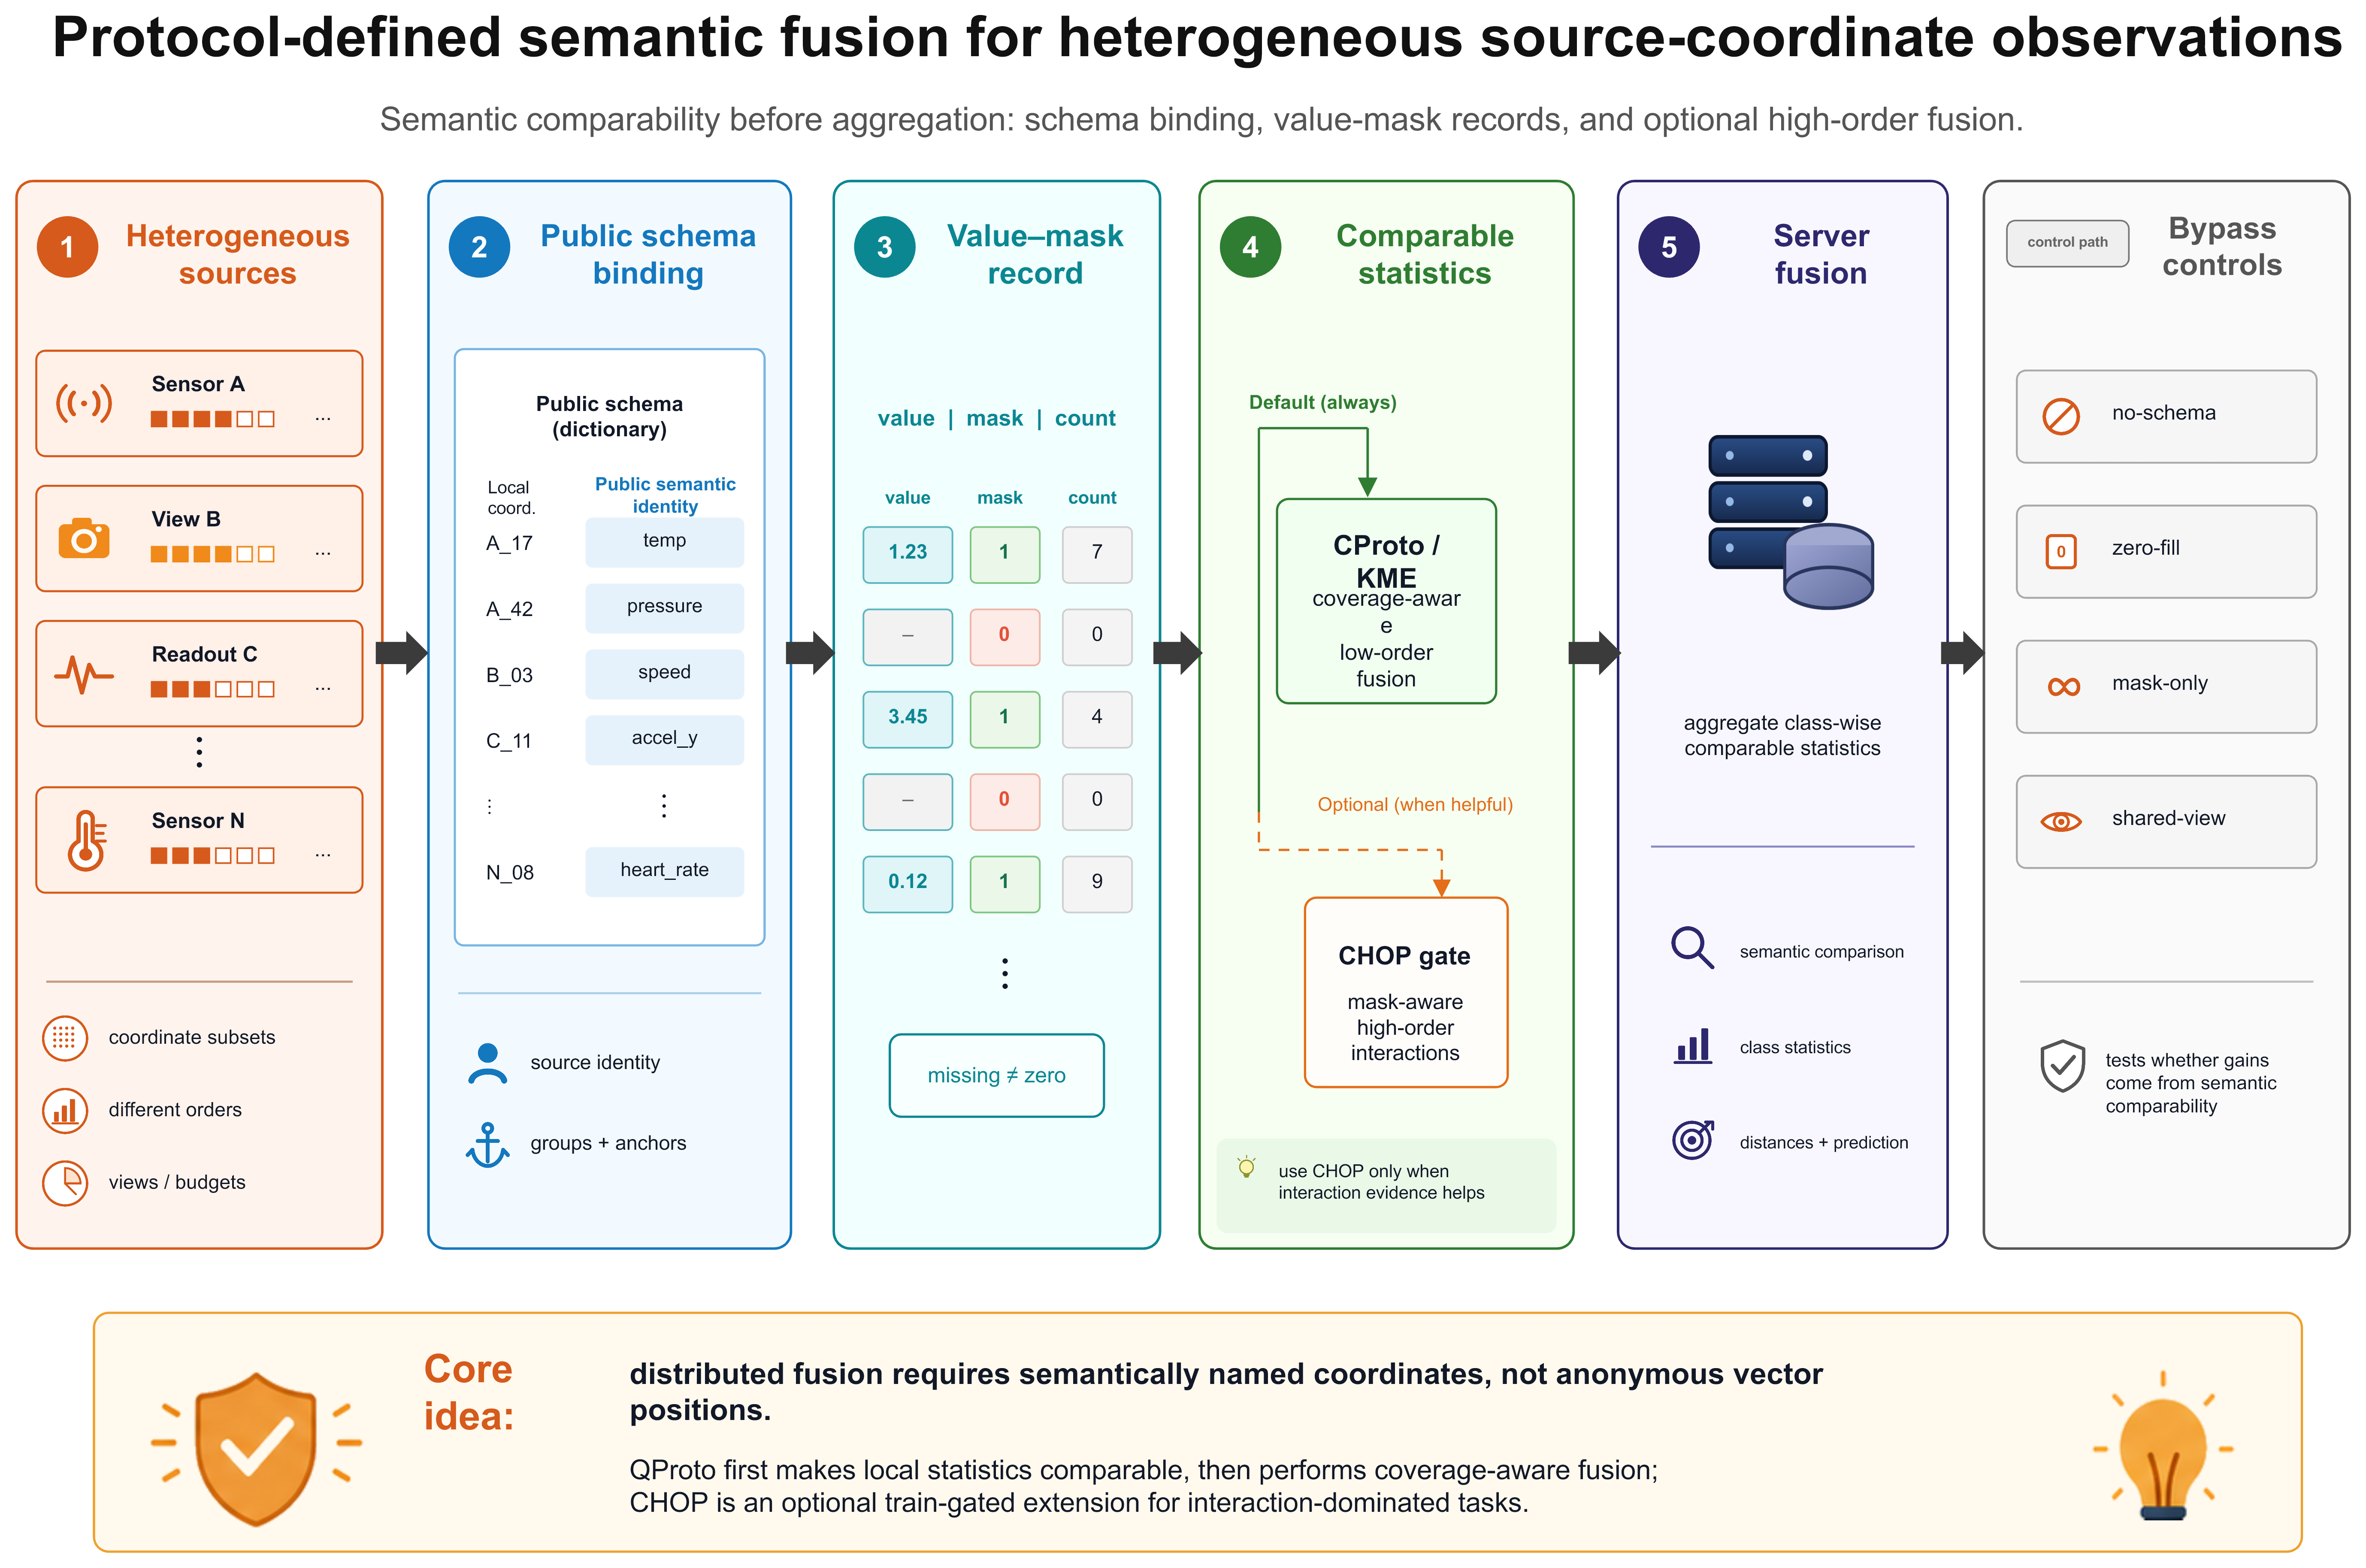
\includegraphics[width=\textwidth]{figures/fig1_semantic_fusion_redrawn_v45_cropped.png}
    \caption{Protocol-defined semantic fusion for heterogeneous source-coordinate observations. Local sources may expose different coordinate subsets, orders, views, noise levels, or measurement budgets. \method\ first binds local coordinates to public semantic identities, then maps observations into value-mask records with coverage counts so that missing measurements are not confused with measured near-zero values. The default path performs low-order coverage-aware CProto/KME fusion, while CHOP is a train-gated high-order extension used only when interaction evidence helps. The bypass controls test whether gains come from semantic comparability rather than anonymous vector averaging.}
    \label{fig:if-framework}
\end{figure*}



Operationally, a client first converts its local readout into a public value-and-mask representation. Values store observed expectation estimates; masks say which protocol coordinates were actually measured. This small distinction is essential because a missing observable and an observed expectation near zero should not be fused as the same event. The default server statistic is low-order: either a finite-dimensional kernel mean sketch or a coverage-aware observable prototype that keeps value sums and coverage counts for each public coordinate. When second-order structure is needed, projected mask-aware outer products add a compressed high-order statistic normalized by the visible coordinate subset. We also implement finite-shot variance shrinkage, but it acts as a reliability hook rather than the main contribution.

The experiments are organized to test one question: what breaks when schema, mask, and coverage are not explicit parts of the fusion rule? In MNIST-4, Fashion-MNIST-4, and CIFAR-4 feature experiments with heterogeneous readout, the no-schema, wrong-schema, forced-canonical, FedAvg, and FedProx controls expose the cost of aggregating statistics whose coordinates are not comparable. In the full-class MNIST-10, Fashion-10, and CIFAR-10 evaluations, the coverage-aware \hopmethod\ variant reaches 0.744, 0.662, and 0.454 accuracy, while the IF-style controls rule out explanations based only on schema metadata, zero-imputation, or shared-observable intersection. The non-quantum checks use the same abstraction on UCI HAR smartphone sensors, UCI Multiple Features, MHEALTH/PAMAP2 wearables, Hydraulic Systems condition monitoring, and WDBC biomedical features. CProto reaches 0.753 on UCI HAR under the same payload where zero-fill RFF and shared-view RFF obtain 0.344 and 0.391. On Multiple Features, group-balanced CProto matches view-wise late fusion at 0.949 and reaches 0.876 under a strict compressed payload; random-key low-order compression is also strong there, so the dataset supports schema-aware low-order fusion rather than a universal key-selection advantage. On subject-held-out MHEALTH, adaptive CHOP reaches 0.878 at the same 13,876-byte payload where low-order CProto obtains 0.860; HeMIS reaches 0.889 and is treated as a centralized trainable boundary. On Hydraulic Systems, compact equal-byte CProto/CHOP reach 0.973/0.977 versus 0.833 for shared-view RFF, while HeMIS reaches 0.997. These comparisons delimit the high-order claim. On many image, sensor, multi-view, and biomedical tasks, semantic coverage-aware fusion is the main gain and HOP is not automatically helpful. For interaction-heavy tasks it becomes important: CHOP reaches 0.732 versus 0.358 for matched low-order CProto in the main covariance-sensing benchmark; supplementary PennyLane high-order readouts improve from 0.422 to 0.550 with mask-aware HOP; and a synthetic covariance benchmark reaches 0.808 versus 0.467 for the low-order variant.

The contributions follow the information-fusion logic of the problem. First, we formulate semantic coordinate comparability as a prerequisite for distributed prototype fusion. Second, we introduce the \method\ value-mask and coverage-count backbone for low-order kernel or source prototypes, including source-group normalization when view dimensionalities differ. Third, we add mask-aware \hopmethod/CHOP as a conditional extension for covariance- or interaction-dominated tasks, with a train-calibrated fallback to low-order CProto. Fourth, we give failure-mode and consistency analyses showing why schema mismatch creates non-vanishing semantic bias. The empirical package is deliberately broad: heterogeneous quantum-readout evaluations, real UCI HAR/MFeat/MHEALTH/PAMAP2/Hydraulic/WDBC missing-view fusion, Qiskit Aer/PennyLane compatibility checks, and covariance-dominated stress tests, all with schema, imputation, deep missing-view, FL/QFL, and equal-byte controls.






\section{Related Work}

\subsection{Information Fusion, Missing Views, and Semantic Alignment}

Information fusion has long treated source identity, representation alignment, missing views, uncertainty, and late or intermediate fusion rules as separate but interacting design choices \cite{castanedo2013datafusion,lahat2015multimodal,baltrusaitis2019multimodal,zhao2017multiview}. Quantum readout gives these choices a particularly sharp form. A client readout is only a partial view of a public observable dictionary, and a coordinate is a physical measurement choice--for example a Pauli string, qubit subset, or measurement basis--rather than an arbitrary feature index. Two numerical readout vectors are therefore not safely fusible until the protocol states which physical observable each coordinate estimates.

Incomplete multi-view and missing-modality methods usually repair or bypass missing views through imputation, modality dropout, prompting, reconstruction, graph or matrix completion, or representation sharing \cite{havaei2016hemis,tang2024incomplete,cai2024projected,wu2024missingmodality}. HeMIS-style fusion, for example, learns modality-specific encoders and aggregates available-view embeddings, making it a strong full-dimensional trainable reference \cite{havaei2016hemis}. Multimodal FL adds privacy and client heterogeneity; recent surveys and benchmarks emphasize missing modalities, modality imbalance, and corrupted labels as robustness challenges \cite{lin2023federatedmultimodal,che2023multimodalsurvey,feng2023fedmultimodal,yu2024fedinmm}. We borrow these baselines deliberately. Schema zero-fill corresponds to simple imputation, mask-only asks whether missingness metadata is enough, shared-observable aggregation keeps only the intersection of views, and HeMIS checks the case where a trainable missing-modality architecture sees full feature-level inputs. Quantum readout differs because missingness is induced by measurement design, not by an absent entry in a table. Observable identity must therefore be part of the protocol itself.

This distinction is also why the comparison is not framed as a claim that QProto replaces learned missing-modality models. Many such models are powerful once a centralized training set provides feature-level samples whose modality identities are already known. QProto targets an earlier protocol question: before reconstruction, modality dropout, or late fusion is meaningful, do the transmitted coordinates have shared source identities, and can compact client statistics be fused without confusing a missing coordinate with a measured zero? This makes schema/order binding and coverage counts first-class fusion objects rather than preprocessing details.

\subsection{Federated Learning as Distributed Fusion}

Federated learning is commonly introduced as decentralized optimization, but it is also a privacy-constrained information-fusion problem: the server combines partial client evidence without direct access to the underlying data sources \cite{yang2019federated,kairouz2021advances}. Classical FL usually assumes that the quantities being combined have compatible semantics, for example shared parameters, shared labels, calibrated sensors, or aligned feature spaces. Heterogeneous FL weakens this assumption through non-IID labels, different models, missing modalities, feature anchors, and client-specific feature spaces \cite{li2020fedprox,karimireddy2020scaffold,acar2021feddyn,reddi2021fedopt,rakotomamonjy2024flic,zhou2024fedfa}. In heterogeneous QFL, the units being fused are finite-shot estimates of quantum observables, so the semantic identity of each coordinate is a physical measurement choice. \method\ makes this identity explicit through a public readout schema.

\subsection{Federated Optimization and Prototype Aggregation}

FedAvg remains the standard communication-efficient reference point for FL \cite{mcmahan2017fedavg}. FedProx stabilizes local training with a proximal term \cite{li2020fedprox}; SCAFFOLD uses control variates to reduce client drift \cite{karimireddy2020scaffold}; FedDyn aligns local and global objectives through dynamic regularization \cite{acar2021feddyn}; and FedOpt covers adaptive server optimizers such as FedAdam, FedYogi, and FedAdagrad \cite{reddi2021fedopt}. These methods are about optimization drift or non-IID data. They do not by themselves solve the more basic question of whether the exchanged coordinates refer to the same source.

Prototype-based FL aggregates class representations rather than gradients or full parameters. FedProto shows that class prototypes can handle heterogeneous client models \cite{tan2022fedproto}. Related representation-level FL methods rely on shared embedding dimensions, public heads, or distillation signals. Our setting is stricter: even if two clients upload same-dimensional class prototypes, coordinate \(a\) may correspond to different quantum observables. Thus \method\ should be viewed as a semantic comparability layer for prototype fusion in QFL, not merely as another prototype averaging rule.

\subsection{Quantum Federated Learning}

Quantum FL now includes hybrid quantum-classical models, QNNs, sequence models, quantum data, and privacy-preserving workflows \cite{chen2021fqml,xia2021quantumfed,chehimi2022qfl,chehimi2024fedqlstm,innan2024fedqnn,kumar2023privacy,ren2025towardqfl,ballester2025qflreview}. Most of this literature asks how to train quantum models or aggregate quantum model parameters. We include trainable PennyLane VQC FedAvg/FedProx baselines for that setting, but the question here is different: what may the server aggregate when clients expose different measurement subsets, readout orders, and finite-shot statistics? Such readout-level heterogeneity can arise for VQCs, quantum kernels, shadow-style measurements, or hybrid QNNs.

\subsection{Quantum Kernels, Readout, and Measurement Sketches}

Quantum kernel methods compare data through quantum feature maps and can offer useful inductive biases when the induced geometry is hard to approximate classically \cite{havlicek2019supervised,schuld2019feature,huang2021power}. Classical shadows estimate many quantum observables from randomized measurements and have become a major tool for efficient property prediction \cite{huang2020classicalshadows,hadfield2022locallybiased,bu2024pauli}. Readout-error mitigation and shot-noise-aware estimation similarly emphasize that measurement outcomes are not generic features; they are noisy estimates tied to a specified measurement procedure. \method\ is complementary to these lines. It does not introduce a new quantum feature map, shadow protocol, or mitigation method. Instead, it specifies how heterogeneous readout statistics should be bound to public observable identities before federated fusion.

\subsection{Kernel Mean Embeddings and Random Features}

Kernel mean embeddings represent probability distributions as expectations in reproducing kernel Hilbert spaces \cite{smola2007hilbert,gretton2012mmd}. Random Fourier features approximate shift-invariant kernels with finite-dimensional sketches \cite{rahimi2007random}. \method\ uses these tools to aggregate class-conditional adapted readout distributions with bounded communication. The \hopmethod\ extension adds projected quadratic features, which are useful when second-order class structure matters. The distinction from ordinary KME aggregation is the schema adapter: without a public value-and-mask domain, the empirical distributions being embedded are not distributions over the same space.

\begin{table*}[t]
\centering
\caption{Protocol requirements addressed by neighboring federated, missing-view, and quantum-readout approaches. Src. = semantic source identity; Order = arbitrary local coordinate order; Miss. = missing-zero distinction; Overlap = non-overlapping but schema-identifiable views; Shot = finite-shot/readout noise; HOP = high-order source interactions; Payload = communication-matched statistics. \(\checkmark\) means the requirement is explicit in the method class, \(\triangle\) means it is partially or indirectly supported, and \(\times\) means it is not addressed by the method class.}
\label{tab:method-positioning}
\scriptsize
\setlength{\tabcolsep}{2pt}
\newcolumntype{Y}{>{\centering\arraybackslash}p{0.085\textwidth}}
\begin{tabular}{p{0.24\textwidth}YYYYYYY}
\toprule
Approach & Src. & Order & Miss. & Overlap & Shot & HOP & Payload \\
\midrule
FedAvg, FedProx, FedOpt & \(\times\) & \(\times\) & \(\times\) & \(\times\) & \(\triangle\) & \(\times\) & \(\checkmark\) \\
FedProto / prototype FL & \(\triangle\) & \(\times\) & \(\times\) & \(\triangle\) & \(\times\) & \(\times\) & \(\checkmark\) \\
Feature-heterogeneous FL & \(\triangle\) & \(\triangle\) & \(\checkmark\) & \(\checkmark\) & \(\times\) & \(\triangle\) & \(\checkmark\) \\
Missing-view imputation & \(\triangle\) & \(\triangle\) & \(\checkmark\) & \(\checkmark\) & \(\times\) & \(\triangle\) & \(\times\) \\
Trainable missing-modality fusion & \(\triangle\) & \(\triangle\) & \(\checkmark\) & \(\checkmark\) & \(\times\) & \(\checkmark\) & \(\times\) \\
Mask-aware or late decision fusion & \(\triangle\) & \(\triangle\) & \(\checkmark\) & \(\checkmark\) & \(\times\) & \(\triangle\) & \(\triangle\) \\
Quantum parameter-FL & \(\times\) & \(\times\) & \(\times\) & \(\times\) & \(\triangle\) & \(\times\) & \(\checkmark\) \\
Quantum kernels/shadows & \(\triangle\) & \(\triangle\) & \(\triangle\) & \(\triangle\) & \(\checkmark\) & \(\checkmark\) & \(\triangle\) \\
\method{} & \(\checkmark\) & \(\checkmark\) & \(\checkmark\) & \(\checkmark\) & \(\checkmark\) & \(\triangle\) & \(\checkmark\) \\
\hopmethod{}/CHOP & \(\checkmark\) & \(\checkmark\) & \(\checkmark\) & \(\checkmark\) & \(\checkmark\) & \(\checkmark\) & \(\checkmark\) \\
\bottomrule
\end{tabular}
\end{table*}


\subsection{Positioning}

Table~\ref{tab:method-positioning} summarizes the distinction in protocol terms rather than in broad method names. The closest conceptual neighbors are FedProto, feature-heterogeneous FL, missing-view imputation, mask-aware deep fusion, late fusion, quantum parameter-FL, and measurement-sketch methods. Each covers part of the design space. The novelty of \method\ is not that value-mask vectors or prototypes are individually new; it is the combination required when source identities themselves are heterogeneous: explicit schema/order binding, missing-zero separation, non-overlapping but semantically identified sources, finite-shot communication accounting, and wrong-schema controls. Without schema binding, prototype averaging may be numerically well-defined but semantically meaningless as a fusion operation.

\section{Problem Setting}

We describe the setting using quantum readout as the motivating instance, while the same protocol applies to general source-coordinate fusion whenever clients expose heterogeneous source identities, local orders, or incomplete views. This covers the readout-level view of quantum FL and measurement-sketch settings as well as ordinary multi-source fusion \cite{ren2025towardqfl,huang2020classicalshadows,hadfield2022locallybiased,castanedo2013datafusion}. Concretely, consider \(K\) clients. Client \(i\) owns a local labeled dataset
\begin{equation}
    \cD_i=\{(x_{in},y_{in})\}_{n=1}^{N_i}, \qquad y_{in}\in\{1,\ldots,C\}.
\end{equation}
For an input \(x\), the client applies a quantum model or, more generally, a source readout pipeline and returns finite-shot or noisy estimates of source coordinates. In quantum settings, these estimates are tied to explicit measurement choices rather than anonymous feature columns \cite{havlicek2019supervised,schuld2019feature,huang2020classicalshadows}. The local readout schema is
\begin{equation}
    \schema_i = \{(a,o_{ia})\}_{a=1}^{m_i},
\end{equation}
where \(a\) is the local coordinate and \(o_{ia}\in\cO\) is the protocol source identity, such as a Pauli string, qubit subset, measurement basis, sensor block, feature family, or other public readout key. The public dictionary \(\cO=\{o_1,\ldots,o_D\}\) is shared, but client \(i\) may observe only a subset.

Let \(r_i(x)\in\R^{m_i}\) denote the raw measurement statistic uploaded or used locally by client \(i\). A typical coordinate may be an expectation estimate
\begin{equation}
    \hat{\mu}_{ia}(x)=\frac{1}{S_i}\sum_{s=1}^{S_i} b_{ias}(x),
\end{equation}
where \(b_{ias}(x)\in\{-1,+1\}\) is a measurement outcome and \(S_i\) is the shot count. The finite-shot variance scales as
\begin{equation}
    \operatorname{Var}[\hat{\mu}_{ia}(x)] \approx \frac{1-\mu_{ia}(x)^2}{S_i}.
\end{equation}

\subsection{Fusion View}

From an information-fusion perspective, client \(i\) observes a source-specific view
\begin{equation}
    V_i(x)=\{(\hat{\mu}_{ia}(x),o_{ia})\}_{a=1}^{m_i}
\end{equation}
of an unobserved semantic readout vector over \(\cO\). The observable key \(o_{ia}\) plays the role of source calibration metadata: it states what physical quantity a local measurement estimates. The missingness pattern is therefore structured rather than arbitrary, as in missing-view fusion, but here it can also be induced by measurement design \cite{havaei2016hemis,tang2024incomplete,huang2020classicalshadows}. A client may omit observable \(o_j\) because of hardware constraints, shot budget, commuting-measurement choices, qubit subset limitations, or a deliberately different readout design. A fusion rule must distinguish three cases that look similar in an ordinary vector representation:
\begin{enumerate}
    \item \(o_j\) was measured and its expectation is near zero;
    \item \(o_j\) was not measured by this client;
    \item a local coordinate was assigned to the wrong public observable.
\end{enumerate}
The first case is a valid quantum statistic, the second is a missing-view event, and the third is semantic mismatch. \method\ is designed around this separation.

\subsection{Why Raw Prototype Aggregation Fails}

Suppose each client computes a class prototype by averaging raw readout vectors. If client coordinate \(a\) corresponds to observable \(Z_1\) for one client and \(X_2Z_3\) for another, then the numerical average of coordinate \(a\) has no stable physical meaning. More formally, if two clients use different local permutations \(P_i\) and \(P_j\) of semantic coordinates, then
\begin{equation}
    \frac{1}{2}(P_i p_i + P_j p_j)
    \neq
    P\left(\frac{1}{2}(p_i+p_j)\right)
\end{equation}
for any single shared semantic permutation \(P\), except in degenerate aligned cases. This is the non-canonical aggregation problem.

The goal is therefore not only to reduce communication, but to define a protocol under which client statistics become comparable before aggregation. We require:
\begin{itemize}
    \item a public observable dictionary;
    \item a local-to-public schema map for each client;
    \item an explicit representation of missing observables;
    \item a compact sketch for class-conditional readout distributions;
    \item communication accounting that treats all baselines fairly.
\end{itemize}

\section{The \method\ Protocol}

\subsection{Learning Objective and Estimator View}

The learning problem can be written as nearest-prototype classification in a protocol-defined comparison space. Let \(A_{\schema_i}\) map client \(i\)'s local readout into the public value-mask domain, let \(g(\cdot)\) denote either the low-order sketch \(\phi\) or the concatenated low-/high-order sketch \((\phi,\sqrt{\lambda}\psi)\), and let
\begin{equation}
    \theta_c^\star = \E[g(A_{\schema}(r(x)))\mid y=c]
\end{equation}
be the population class statistic in the common semantic domain. The server estimates \(\theta_c^\star\) from client-local empirical statistics without observing raw examples:
\begin{equation}
    \hat{\theta}_c =
    \sum_i
    \frac{|\cD_{i,c}|}{\sum_\ell |\cD_{\ell,c}|}
    \hat{\theta}_{i,c}.
\end{equation}
Prediction minimizes the plug-in risk induced by prototype distances,
\begin{equation}
    \hat{y}(x)=
    \arg\min_c
    \|g(A_{\schema}(r(x)))-\hat{\theta}_c\|_2^2.
\end{equation}
This viewpoint matters because schema binding is part of the statistical model. Without \(A_{\schema_i}\), the client estimates are not samples from a shared random variable. It also separates the roles of the modules: low-order \(\phi\) estimates class mean embeddings, coverage-aware prototypes estimate observable-wise conditional means with missingness counts, and HOP estimates projected second-order moments. Unless stated otherwise, CProto is the default compact backbone; CHOP is a conditional branch for interaction-heavy regimes, not a replacement for low-order coverage fusion.

\subsection{Protocol Summary}

The protocol used in the experiments is:
\begin{enumerate}
    \item Define a public observable dictionary \(\cO\), optional public anchors, sketch dimensions, and communication budget.
    \item For each client \(i\), bind every local measurement coordinate to a public observable identity through \(\schema_i\).
    \item Locally measure finite-shot readout statistics and map them to the public value-mask domain \(A_{\schema_i}(r_i(x))\).
    \item Estimate class-wise low-order statistics, coverage counts, and, when enabled, mask-aware high-order sketches.
    \item Upload only the protocol statistics, not raw examples or full measurement records.
    \item Aggregate class statistics by class counts and compare test readouts in the same public comparison domain.
\end{enumerate}
The second step is the one the paper is built around. If local coordinates are not bound to public observable identities, the remaining steps may still produce vectors, but they no longer define a valid fusion estimator.

\subsection{Schema Adapter}

For client \(i\), the schema adapter maps a raw local readout vector to a public comparison vector:
\begin{equation}
    A_{\schema_i}: \R^{m_i}\rightarrow \R^{2D}.
\end{equation}
The first \(D\) coordinates store observable values and the second \(D\) coordinates store a missingness mask. For public observable \(o_j\),
\begin{equation}
    [A_{\schema_i}(r)]_j =
    \begin{cases}
        r_a, & \text{if } o_{ia}=o_j \text{ for some } a,\\
        0, & \text{otherwise},
    \end{cases}
\end{equation}
and
\begin{equation}
    [A_{\schema_i}(r)]_{D+j} =
    \mathbf{1}\{o_j \text{ is measured by client } i\}.
\end{equation}
The mask is what keeps an unmeasured coordinate from being treated as a measured expectation near zero.

\subsection{Low-Order Kernel Sketches}

Let \(z=A_{\schema_i}(r_i(x))\). We use a random Fourier feature map
\begin{equation}
    \phi(z)=\sqrt{\frac{2}{d}}\cos(Wz+b)\in\R^d,
\end{equation}
where rows of \(W\) are sampled according to a shift-invariant kernel and \(b\) is uniform on \([0,2\pi]\), following the standard random-feature approximation of kernel values \cite{rahimi2007random}. Public anchors may be used to estimate coordinate centers and scales, but our current results suggest that naive anchor normalization should be treated carefully.

Client \(i\)'s low-order class prototype is
\begin{equation}
    \mu_{i,c} =
    \frac{1}{|\cD_{i,c}|}\sum_{(x,y)\in\cD_i:y=c}
    \phi(A_{\schema_i}(r_i(x))).
\end{equation}
This approximates a kernel mean embedding of the class-conditional adapted readout distribution \cite{smola2007hilbert,gretton2012mmd}.

\subsection{Coverage-Aware Observable Prototypes}

The value-mask sketch is compact, but it can hide an important feature of heterogeneous readout: an observable may be measured by only a subset of clients, and that coverage pattern is protocol information. We therefore include a coverage-aware variant, denoted \method{}-Masked, that aggregates observable identities directly before any high-order extension.

Write the adapted value and mask coordinates as \(v_j(x)\) and \(m_j(x)\). Client \(i\) uploads, for each class \(c\) and observable \(j\),
\begin{equation}
    S_{i,cj}=\sum_{(x,y)\in\cD_i:y=c}m_j(x)v_j(x),
    \qquad
    N_{i,cj}=\sum_{(x,y)\in\cD_i:y=c}m_j(x).
\end{equation}
The server forms the coverage-aware class prototype
\begin{equation}
    \bar v_{cj}=
    \frac{\sum_i S_{i,cj}}{\sum_i N_{i,cj}+\epsilon}.
\end{equation}
Prediction compares a test readout only on coordinates that are both observed by the test schema and covered by the class prototype:
\begin{equation}
    d_c(x)=
    \frac{
    \sum_j m_j(x)\mathbf{1}\{N_{cj}>0\}w_{cj}
    (v_j(x)-\bar v_{cj})^2
    }{
    \sum_j m_j(x)\mathbf{1}\{N_{cj}>0\}w_{cj}+\epsilon
    },
\end{equation}
where \(w_{cj}\) is a mild coverage weight. This variant is less compressed than the RFF prototype but directly tests the central claim of the paper: once observable identities are protocol-bound, non-shared but semantically comparable readouts can still contribute to aggregation.

When protocol sources are naturally grouped, as in multi-sensor or multi-view benchmarks, a coordinate-wise distance can overweight high-dimensional sources. We therefore include a source-normalized scoring option that first computes the coverage-aware distance inside each semantic group \(G_q\) and then averages over observed groups:
\begin{equation}
    d_c^{\mathrm{grp}}(x)=
    \frac{1}{|\mathcal{Q}_x|}
    \sum_{q\in\mathcal{Q}_x}
    \frac{\sum_{j\in G_q} m_j(x)\mathbf{1}\{N_{cj}>0\}w_{cj}(v_j(x)-\bar v_{cj})^2}
    {\sum_{j\in G_q} m_j(x)\mathbf{1}\{N_{cj}>0\}w_{cj}+\epsilon}.
\end{equation}
Group-balanced CProto is unnecessary when all public observables are exchangeable. It becomes important in information-fusion settings where one source contributes many more coordinates than another.

\subsection{\hopmethod: Mask-Aware High-Order Outer-Product Sketches}

Low-order sketches may be weak when classes have similar means but different covariance or higher-order geometry, a regime where second-order statistics can separate distributions that share first-order moments. The \hopmethod\ extension computes a high-order sketch over the adapted value vector \(v\in\R^D\), excluding the mask as a direct feature but using it to normalize projections:
\begin{equation}
    \psi_k(v,m)=
    \left(
    \frac{p_k^\top(m\odot v)}
    {\sqrt{p_k^\top \operatorname{diag}(m)p_k+\epsilon}}
    \right)^2,
    \qquad k=1,\ldots,h,
\end{equation}
where \(p_k\) is the \(k\)-th random projection vector. If all observables are visible, this reduces to the usual projected outer-product statistic \((p_k^\top v)^2\). Under heterogeneous readout, the denominator prevents high-order coordinates from changing scale merely because a client observed fewer protocol observables.

The client uploads
\begin{equation}
    H_{i,c} =
    \frac{1}{|\cD_{i,c}|}\sum_{(x,y)\in\cD_i:y=c}\psi(v_i(x),m_i(x)).
\end{equation}
HOP is therefore not appended after alignment; it is a high-order statistic defined inside the same comparability protocol.

\subsection{When to Use HOP}

The high-order branch is not the default estimator. The default compact statistic is CProto, because many heterogeneous-source tasks are separable by low-order coverage-aware evidence once coordinate identities are correct. HOP is enabled only when there is training-only evidence that pairwise or covariance structure carries class information. In practice this means one of two conditions holds: the public-anchor score selects stable cross-source pairs with nontrivial variation, or the calibration split shows that a CHOP mixture improves over the low-order branch under the same payload. If neither condition holds, adaptive CHOP falls back to CProto.

This rule is part of the method rather than a post-hoc interpretation. It prevents the paper from treating quadratic sketches as universally beneficial, and it makes the high-order claim falsifiable: HOP should help on interaction-dominated benchmarks and should be neutral or disabled on low-order, imputation-friendly benchmarks. The experiments therefore report CProto, CHOP, adaptive CHOP, random-key HOP, and equal-byte RFF controls together.

\subsection{Compressed Coverage-Aware HOP}

The full coverage-aware protocol communicates statistics for all \(D\) public observables. To test whether the high-order gain survives under tighter communication, we add a compressed variant, CHOP. A public anchor set is measured under the client schemas, and the protocol selects \(K<D\) observable keys using an anchor-informed unsupervised score, such as coverage
\begin{equation}
    s^{\mathrm{cov}}_j = \widehat{\Pr}(m_j=1)
\end{equation}
or coverage-weighted variation
\begin{equation}
    s^{\mathrm{var}}_j =
    \widehat{\mathrm{Var}}(v_j)\sqrt{\widehat{\Pr}(m_j=1)}.
\end{equation}
The client then sends coverage-aware value sums, coverage counts, and mask-aware HOP statistics only for the selected key set \(\cK\). A compressed low-order control, denoted CProto, uses the same key set without HOP. This makes the HOP comparison strict: CHOP and CProto differ by the high-order sketch, not by the selected observables. Random-key controls check that CHOP is not simply benefiting from arbitrary \(K\)-coordinate compression.

\subsection{Adaptive High-Order Gate}

Because high-order statistics are useful only when the task contains source interactions, we also define an adaptive CHOP variant. Each client reserves a small training-only calibration split. The low-order equal-byte CProto branch and the CHOP statistics are fitted on the remaining training data. The calibration split is then used to choose among a small budget-matched candidate set: the low-order CProto branch and CHOP mixtures
\begin{equation}
    d_c^{(\alpha)}(z)=
    \alpha d^{\mathrm{low}}_c(z)
    +(1-\alpha)\lambda d^{\mathrm{hop}}_c(z),
    \qquad
    \alpha\in\{0,0.25,0.5,0.75,1\}.
\end{equation}
Clients evaluate these candidates under their own schemas and report only aggregate calibration scores. The protocol uses a CHOP mixture only when its calibration accuracy exceeds the low-order branch by a margin \(\tau\); otherwise it falls back to equal-byte CProto. The selected candidate is then refit on the full training data before test evaluation. No test labels are used, and all candidates fit inside the same per-round payload budget. The gate is not meant to make HOP universally dominant. Its purpose is narrower: avoid high-order sketches on low-order-separable tasks and retain CHOP mixtures on interaction-dominated tasks.

\subsection{Server Aggregation}

For each class \(c\), the server aggregates local statistics by class counts:
\begin{equation}
    \mu_c = \sum_i \alpha_{i,c}\mu_{i,c},\qquad
    H_c = \sum_i \alpha_{i,c}H_{i,c},
\end{equation}
where
\begin{equation}
    \alpha_{i,c}=
    \frac{|\cD_{i,c}|}{\sum_j |\cD_{j,c}|}.
\end{equation}
At prediction time, a test readout from schema \(\schema\) is adapted to \(z\), sketched to \(\phi(z)\), and compared to class prototypes:
\begin{equation}
    d_c(z)=
    \|\phi(z)-\mu_c\|_2^2
    + \lambda \|\psi(v)-H_c\|_2^2.
\end{equation}
The predicted label is \(\arg\min_c d_c(z)\). Setting \(\lambda=0\) recovers the low-order prototype variant.

\subsection{Optional Shot-Variance Shrinkage}

Finite shots provide a measurable uncertainty proxy. We estimate client reliability as
\begin{equation}
    \rho_i = \frac{1}{1+\gamma\sigma_i^2},
    \qquad
    \sigma_i^2 \approx
    \frac{1}{B}\sum_{x,a}\frac{1-\hat{\mu}_{ia}(x)^2}{S_i}.
\end{equation}
The server may shrink noisy local statistics before aggregation. In our experiments, this module is mixed on real image tasks and should be viewed as optional. The main method is the comparability protocol plus low-order kernel prototypes; HOP and shrinkage are extensions for specific regimes.

\subsection{Communication}

For scalar size \(b\), \(C\) classes, low-order dimension \(d\), and high-order dimension \(h\), the per-client per-round payload is
\begin{equation}
    \mathcal{B} \approx b\,C(d+h+1) + O(b),
\end{equation}
with \(h=0\) for prototype-only variants. The implementation records bytes per client per round and includes matched communication controls.
For \method{}-Masked with \(D\) protocol observables, the payload is approximately
\begin{equation}
    \mathcal{B}_{\mathrm{mask}}
    \approx b\,\{C(2D+1)+1\},
\end{equation}
because each client sends value sums and coverage counts. We therefore report matched-budget controls where low-order RFF and shared-observable baselines receive the same byte budget.
For CHOP with \(K\) selected observables and HOP dimension \(h\),
\begin{equation}
    \mathcal{B}_{\mathrm{CHOP}}
    \approx b\,\{C(2K+h+1)+1\}.
\end{equation}
Adaptive CHOP uses the same accounting as its selected candidate: either the equal-byte CProto fallback or the fixed CHOP payload with a chosen mixture weight. The calibration decision itself is a protocol choice and does not add per-class prototype statistics.

\section{Analysis}

This section gives the formal pieces needed for the paper's main claim. The results are deliberately modest. They do not claim a hardware-independent quantum advantage; they show that schema mismatch creates an irreducible semantic error, while correct schema binding turns aggregation into concentration of comparable distributional statistics. The supplement adds the longer plug-in margin argument, group-balanced scoring analysis, adaptive-CHOP calibration bound, and finite-budget error decomposition.

\begin{assumption}[Bounded adapted readouts]
For every client \(i\), input \(x\), and observable key \(o_j\), the adapted readout value satisfies \(|v_{ij}(x)|\le 1\), and the mask coordinate is binary. The kernel \(k\) is bounded by one and is approximated by \(d\) random Fourier features.
\end{assumption}

\begin{assumption}[Correct schema model]
There exists a public observable dictionary \(\cO=\{o_1,\ldots,o_D\}\). Under correct schema, every local coordinate maps to its true public observable key. Under wrong schema, at least one positive-mass observable subset is mapped to an incorrect key.
\end{assumption}

\begin{assumption}[Regular sketches]
The low-order feature map \(\phi\) and the HOP feature map \(\psi\) are bounded and Lipschitz on the adapted readout domain. For random feature dimension \(d\) and HOP dimension \(h\), their approximation errors satisfy the usual Monte Carlo rates \(O(d^{-1/2})\) and \(O(h^{-1/2})\) with high probability.
\end{assumption}

\subsection{Schema Mismatch Lower Bound}

\begin{theorem}[Irreducible schema mismatch error]
Consider two clients with class-conditional semantic prototypes \(p_{1,c},p_{2,c}\in\R^D\). If client 2 uses a wrong schema permutation \(P\neq I\) and the server averages in the reported coordinates, then there exist class distributions with identical sample size and zero measurement noise such that the aggregated prototype differs from the correct semantic prototype by
\begin{equation}
    \left\|
    \frac{p_{1,c}+Pp_{2,c}}{2}
    -
    \frac{p_{1,c}+p_{2,c}}{2}
    \right\|_2
    \ge
    \frac{1}{2}\|(P-I)p_{2,c}\|_2.
\end{equation}
The error persists as the number of samples, shots, and sketch dimension go to infinity whenever \(p_{2,c}\) is not in the fixed subspace of \(P\).
\end{theorem}

\begin{proof}
With infinite samples and noiseless measurements, both clients recover their population semantic prototypes exactly. The correct aggregate is \((p_{1,c}+p_{2,c})/2\). If client 2 reports coordinates through \(P\), the server forms \((p_{1,c}+Pp_{2,c})/2\). Subtracting the two aggregates gives \((P-I)p_{2,c}/2\), so the displayed norm follows with equality. The right-hand side is independent of sample size, shot budget, and sketch dimension. It is nonzero whenever \(p_{2,c}\notin\mathrm{Fix}(P)\).
\end{proof}

\subsection{Correct-Schema Consistency}

\begin{theorem}[Consistency of comparable kernel prototypes]
Under the correct schema model and bounded readouts, let
\begin{equation}
    \mu_c^\star=\E_{z\sim P_c}[\phi(z)]
\end{equation}
be the class-\(c\) mean in the public value-mask domain for the finite feature map. If class samples are independent and all clients use the adapter \(A_{\schema_i}\), then the aggregated prototype \(\hat{\mu}_c\) is a consistent estimator of \(\mu_c^\star\). If the comparison is made to the infinite-dimensional kernel mean embedding, then with probability at least \(1-\delta\),
\begin{equation}
    \|\hat{\mu}_c-\mu_c^\star\|_2
    \le
    C\!\left(
    \sqrt{\frac{\log(1/\delta)}{n_c}}
    +
    \sqrt{\frac{\log(1/\delta)}{d}}
    +
    \sqrt{\frac{\log(1/\delta)}{S_{\min}}}
    \right),
\end{equation}
where \(n_c\) is the total number of class-\(c\) examples, \(d\) is the RFF dimension, \(S_{\min}\) is the minimum shot budget, and \(C\) depends on the bounded-domain and Lipschitz constants.
\end{theorem}

\begin{proof}
Under correct schema, every local readout is first mapped into the same public value-mask space. Thus the server average is a class-count-weighted empirical mean of comparable random variables \(\phi(z)\). The boundedness assumption gives a vector-valued concentration term of order \(O(\sqrt{\log(1/\delta)/n_c})\). If one compares the finite RFF mean to the exact kernel mean, standard random-feature concentration contributes \(O(\sqrt{\log(1/\delta)/d})\). Finally, each adapted expectation is an average of bounded measurement outcomes, so finite shots perturb the readout by \(O(\sqrt{\log(1/\delta)/S_{\min}})\); Lipschitzness of \(\phi\) transfers this perturbation to the feature mean. Union-bounding the three deviations yields the result. There is no schema-mismatch term because all coordinates are aggregated under their public observable identities.
\end{proof}

\begin{theorem}[One explicit finite-budget form]
\label{thm:finite-budget}
Let \(m=2D\) be the value-mask dimension, let \(\|\phi(z)\|_2\le R_\phi\), and let \(\phi\) be \(L_\phi\)-Lipschitz. Assume each observed Pauli expectation is estimated from at least \(S_{\min}\) independent shots and each class has \(n_c\) total examples after client aggregation. For a fixed query point and a fixed class \(c\), the score error between the empirical finite-shot RFF prototype and the population exact-kernel prototype is bounded with probability at least \(1-\delta\) by
\begin{equation}
\begin{aligned}
    |\widehat{s}_c(z)-s_c^\star(z)|
    \le&
    2R_\phi^2\sqrt{\frac{2\log(6/\delta)}{n_c}}
    +2R_\phi L_\phi
    \sqrt{\frac{2D\log(6D/\delta)}{S_{\min}}}  \\
    &+
    2\sqrt{\frac{2\log(6/\delta)}{d}} .
\end{aligned}
\end{equation}
Consequently, if the population class-margin exceeds twice the right-hand side uniformly over competing classes, nearest-prototype classification is unchanged by finite samples, finite shots, and finite RFF dimension.
\end{theorem}

\begin{proof}
Decompose the score error into three terms: empirical prototype concentration for bounded vectors, perturbation of the adapted readout caused by finite-shot measurement, and random-feature approximation of the exact kernel score. The first term follows from Hilbert-space Hoeffding for vectors bounded by \(R_\phi\). For the second term, Hoeffding applied to \(D\) Pauli expectation estimates gives \(\|\tilde z-z\|_2\le\sqrt{2D\log(6D/\delta)/S_{\min}}\) with high probability; Lipschitzness of \(\phi\) and the bound \(\|\phi\|\le R_\phi\) convert this to score error. The third term is the standard bounded random-feature Monte Carlo error for a fixed pair. A union bound over the three events gives the displayed inequality. The margin statement follows by comparing every incorrect-class score to the correct-class score.
\end{proof}

\subsection{Coverage-Aware Value/Count Estimation}

\begin{theorem}[Coverage-aware prototype bias and variance]
\label{thm:coverage-estimator}
Fix a class \(c\) and public source coordinate \(j\). Let \(M_{ij}\in\{0,1\}\) indicate whether client \(i\) observes coordinate \(j\), and let \(V_{ij}\in[-1,1]\) be the corresponding adapted value for samples in class \(c\). The coverage-aware estimator
\begin{equation}
    \hat{m}_{cj}
    =
    \frac{\sum_i\sum_{\ell:y_{i\ell}=c}M_{ij\ell}V_{ij\ell}}
    {\sum_i\sum_{\ell:y_{i\ell}=c}M_{ij\ell}}
\end{equation}
is unbiased for \(m_{cj}=\E[V_j\mid y=c,M_j=1]\). If the missingness mechanism is conditionally source-independent, \(M_j\perp V_j\mid y=c\), then \(m_{cj}=\E[V_j\mid y=c]\). Conditional on \(N_{cj}\) observed class-\(c\) values for coordinate \(j\),
\begin{equation}
    \Pr(|\hat{m}_{cj}-m_{cj}|>\epsilon\mid N_{cj})
    \le 2\exp(-N_{cj}\epsilon^2/2).
\end{equation}
\end{theorem}

\begin{proof}
The estimator is an empirical mean over the observed class-\(c\) values for source \(j\), so unbiasedness for \(\E[V_j\mid y=c,M_j=1]\) follows directly. Under conditional source-independent missingness, the observed and full class-conditional value distributions coincide. Since \(V_j\in[-1,1]\), Hoeffding's inequality gives the displayed conditional concentration bound. Thus the variance term is controlled by coverage count \(N_{cj}\), which motivates storing value sums and observation counts separately rather than imputing missing coordinates as zero.
\end{proof}

\begin{theorem}[Partially incorrect schema metadata]
\label{thm:noisy-schema}
Suppose a fraction \(\rho_{ij}\) of observed coordinate assignments for source \(j\) are mapped to incorrect public keys, and assume \(|V_{ij}|\le1\). Let \(\hat{m}_{cj}^{\mathrm{noisy}}\) be the coverage-aware estimator formed with this noisy schema and \(\hat{m}_{cj}^{\mathrm{clean}}\) the estimator formed with the true schema on the same observations. Then
\begin{equation}
    |\E[\hat{m}_{cj}^{\mathrm{noisy}}]-\E[\hat{m}_{cj}^{\mathrm{clean}}]|
    \le 2\rho_{cj},
\end{equation}
where \(\rho_{cj}\) is the class-\(c\) observed mass assigned to an incorrect key for coordinate \(j\). The error does not vanish with additional samples unless \(\rho_{cj}\to0\).
\end{theorem}

\begin{proof}
Incorrect schema assignments replace some values whose correct coordinate is \(j\) with values from other coordinates, or move true \(j\)-values away from coordinate \(j\). Since all values are bounded in \([-1,1]\), replacing a \(\rho_{cj}\) fraction of the observed mass can change the coordinate mean by at most \(2\rho_{cj}\). This is a semantic-bias term, not a sampling term. More samples reduce variance around the wrong semantic mean but do not remove the bias.
\end{proof}

\subsection{Finite-Shot Propagation}

\begin{theorem}[Finite-shot effect on prototype distances]
Let \(\tilde{z}=z+\eta\) be an adapted readout with finite-shot noise and assume \(\phi\) is \(L_\phi\)-Lipschitz on the bounded readout domain. Then for any class prototype \(\mu_c\),
\begin{equation}
    \left|
    \|\phi(\tilde{z})-\mu_c\|_2^2
    -
    \|\phi(z)-\mu_c\|_2^2
    \right|
    \le
    2R L_\phi\|\eta\|_2 + L_\phi^2\|\eta\|_2^2,
\end{equation}
where \(R\) bounds \(\|\phi(z)-\mu_c\|_2\). In expectation, the leading term scales as \(O(S^{-1/2})\).
\end{theorem}

\begin{proof}
Let \(a=\phi(z)-\mu_c\) and \(\Delta=\phi(\tilde z)-\phi(z)\). Then
\begin{equation}
    \|a+\Delta\|_2^2-\|a\|_2^2=2a^\top\Delta+\|\Delta\|_2^2.
\end{equation}
Taking absolute values and using Cauchy--Schwarz gives \(2\|a\|_2\|\Delta\|_2+\|\Delta\|_2^2\). Since \(\|a\|_2\le R\) and \(\|\Delta\|_2\le L_\phi\|\eta\|_2\), the displayed bound follows. For bounded \(\{-1,+1\}\) measurement outcomes, \(\E\|\eta\|_2=O(S^{-1/2})\) up to dimension and coverage constants, giving the leading shot term.
\end{proof}

\subsection{High-Order Separability}

\begin{theorem}[Random quadratic sketches separate covariance differences]
Let two classes have adapted value distributions with equal mean but covariance matrices \(\Sigma_1\neq\Sigma_2\). For a random projection vector \(p\), the HOP statistic satisfies
\begin{equation}
    \E[(p^\top v)^2\mid y=1]
    -
    \E[(p^\top v)^2\mid y=2]
    =
    p^\top(\Sigma_1-\Sigma_2)p.
\end{equation}
If \(\|\Sigma_1-\Sigma_2\|_F>0\), then with nonzero probability over \(p\), the projected quadratic statistic separates the classes. With \(h\) independent projections, the probability of missing all nonzero covariance directions decays exponentially in \(h\) under standard sub-Gaussian projection assumptions.
\end{theorem}

\begin{proof}
Because the class means are equal, the difference in projected second moments is
\begin{equation}
    \E[(p^\top v)^2\mid y=1]-\E[(p^\top v)^2\mid y=2]
    =p^\top(\Sigma_1-\Sigma_2)p.
\end{equation}
Let \(A=\Sigma_1-\Sigma_2\). For an isotropic Gaussian projection, \(\E[(p^\top A p)^2]=2\|A\|_F^2+(\mathrm{tr}\,A)^2\), which is positive when \(A\neq0\). Hence a single projection has positive probability of producing a nonzero high-order gap. For independent projections, the probability that all projected gaps fall below a fixed detectable threshold is the product of the individual miss probabilities and therefore decays exponentially in \(h\). This is the regime in which \hopmethod\ should help: covariance-dominated tasks, not low-order-separable image tasks.
\end{proof}

\subsection{Anchor-Informed CHOP Key Selection}

CHOP uses public anchors only to choose a compact set of observable keys or quadratic pairs before private client aggregation begins. The selection rule is not claimed to be optimal. Its role is narrower: if the public anchor distribution overlaps source coordinates whose class-conditional variance or covariance is informative, then variance- or covariance-ranked keys are more likely than uniformly random keys to keep useful coordinates. This is a sufficient-condition argument, not a universal guarantee. The random-key ablations are therefore essential: they test whether the selected keys carry semantic signal beyond compression alone.

\subsection{Communication-Error Trade-Off}

\begin{theorem}[Budget allocation between low-order and high-order sketches]
Suppose the sketch contribution to the classification margin error is bounded by
\begin{equation}
    \epsilon(d,h)\le a d^{-1/2}+c h^{-1/2},
\end{equation}
where \(a\) measures low-order signal difficulty and \(c\) measures high-order signal difficulty. Under a payload constraint \(bC(d+h+1)\le B\), the continuous relaxation allocates
\begin{equation}
    \frac{h}{d}=\left(\frac{c}{a}\right)^{2/3}.
\end{equation}
\end{theorem}

\begin{proof}
Let \(M=B/(bC)-1\), so \(d+h\le M\). At the optimum the budget is active. Minimize \(a d^{-1/2}+c h^{-1/2}\) subject to \(d+h=M\). The Lagrange conditions give
\begin{equation}
    a d^{-3/2}=c h^{-3/2},
\end{equation}
which rearranges to \(h/d=(c/a)^{2/3}\). The empirical communication curves follow this qualitative rule: low-order image tasks benefit more from low-order allocation, whereas covariance-dominated readout benefits from allocating payload to HOP.
\end{proof}

\section{Experiments}
\label{sec:experiments}

\subsection{Experimental Design}

The experiments are organized around three questions rather than a single leaderboard. Does a fusion rule fail when source coordinates are not semantically comparable? Is value/count coverage enough to recover useful low-order evidence from non-shared but identifiable sources? When the signal is genuinely interaction-heavy, does a mask-aware high-order statistic add anything beyond CProto?

For the quantum-readout experiments, every client measures only a subset of a public latent observable dictionary and may use its own local coordinate order. Shot count, readout noise, depolarizing attenuation, and circuit depth can also differ. The non-quantum benchmarks keep the same abstraction but replace Pauli observables with named sensor or biomedical feature groups. In both cases, the server treats two coordinates as comparable only after the schema adapter supplies the public source identity. The supplementary protocol manifest records the client splits, seeds, source dictionaries, schema sampling, public-anchor construction, tuning data, and payload accounting for each benchmark.
The supplement begins with a claim-to-evidence map that links each experiment to the same failure mode: what changes when schema, mask, coverage, or interaction statistics are removed from the fusion protocol.

\subsection{Core Baselines}

The main tables use baselines as diagnostic instruments rather than as one undifferentiated leaderboard. We separate three groups. First, no-schema, forced-canonical, wrong-schema, mask-only metadata, schema zero-fill, and shared-view aggregation test semantic mismatch, missingness metadata, and view-intersection explanations. Second, equal-byte RFF, CProto, group CProto, CHOP, and adaptive CHOP form the communication-matched compact-statistic comparisons. Third, mean/PCA/ridge imputation, anchor autoencoder imputation, mask-aware pooled MLP, HeMIS-style modality-dropout fusion, and view-wise late fusion are full-dimensional or trainable boundary references when centralized feature-level training is allowed. FedProto/FedOpt-style rows test familiar FL alternatives. All named baselines are local adaptations run under the same train/test splits, schema sampling, payload accounting, and source dictionaries used by the corresponding QProto row; we do not import numerical accuracies from the original papers, whose datasets, objectives, and visibility assumptions differ from this protocol. This grouping is important: QProto is not presented as a universal replacement for deep missing-modality models, but as a compact schema-aware protocol when source identity and payload constraints matter. The supplementary material contains the additional QFL optimizer, backend, scale, shot-noise, and communication sweeps.

Figure~\ref{fig:main-results-overview} summarizes the main empirical pattern across full-class heterogeneous readout, real missing-view fusion, high-order source interactions, and circuit-generated readout compatibility.

\begin{figure*}[t]
    \centering
    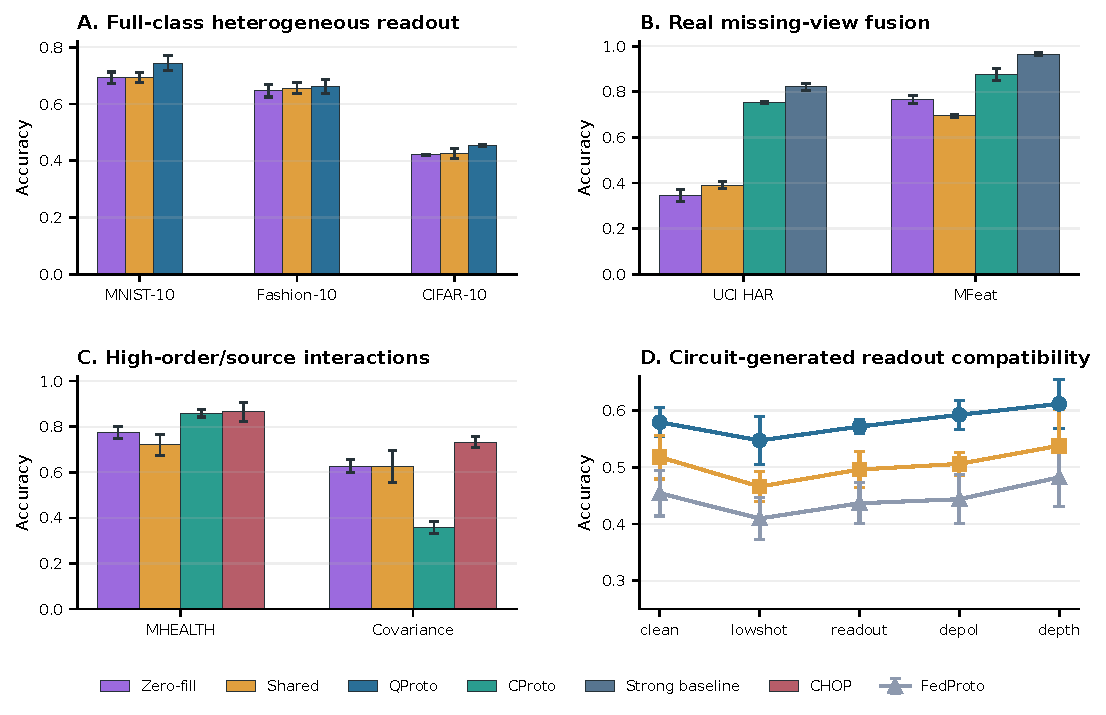
\includegraphics[width=0.98\textwidth]{if_main_result_overview.pdf}
    \caption{Main empirical picture. QProto improves over zero-fill/shared-view controls on full-class readout and real missing-view tasks. In panel B, Strong baseline denotes the full-dimensional HeMIS-style modality-dropout fusion reference. Panel C pairs the real MHEALTH wearable source-interaction benchmark with the controlled covariance benchmark. Qiskit Aer count-derived readouts provide circuit-generated compatibility evidence, not hardware validation.}
    \label{fig:main-results-overview}
\end{figure*}

\subsection{Real Non-Quantum Missing-View Fusion}

\begin{table*}[t]
\centering
\caption{Real non-quantum missing-view fusion benchmark on UCI HAR smartphone-sensor features. Feature-name groups are treated as semantic sensor views; each client observes a heterogeneous subset. Equal-byte rows use the same per-client per-round payload as CHOP.}
\label{tab:if-nonquantum-fusion}
\scriptsize
\setlength{\tabcolsep}{3pt}
\renewcommand{\arraystretch}{0.94}
\begin{tabular}{lcccc}
\toprule
Method & Acc. & 95\% CI & Bytes & Runtime (s) \\
\midrule
Mask-only metadata & 0.163 & 0.005 & 13492 & 1.063 \\
Zero-fill prototype & 0.275 & 0.035 & 13492 & 1.057 \\
Mean-impute prototype & 0.569 & 0.032 & 13492 & 1.497 \\
Value+mask prototype & 0.208 & 0.036 & 26956 & 2.050 \\
Anchor PCA imputation & 0.779 & 0.012 & 13492 & 26.368 \\
Learned ridge imputation & 0.770 & 0.016 & 13492 & 3.486 \\
Anchor autoencoder imputation & 0.753 & 0.005 & 13492 & 14.623 \\
Mask-aware pooled MLP & 0.757 & 0.022 & 26956 & 4.778 \\
HeMIS modality-dropout fusion & 0.821 & 0.023 & 26956 & 32.261 \\
View-wise late fusion & 0.717 & 0.017 & 13492 & 0.294 \\
Shared-view prototype & 0.391 & 0.021 & 52 & 0.013 \\
Shared-view RFF equal bytes & 0.391 & 0.021 & 7708 & 0.647 \\
Zero-fill RFF equal bytes & 0.344 & 0.038 & 7708 & 1.204 \\
Coverage prototype all & 0.781 & 0.003 & 26956 & 2.136 \\
Group-balanced CProto all & 0.717 & 0.017 & 26956 & 2.407 \\
CProto equal bytes & 0.753 & 0.009 & 7708 & 0.545 \\
Group-balanced CProto equal bytes & 0.716 & 0.016 & 7708 & 0.571 \\
Random-key CProto equal bytes & 0.632 & 0.033 & 7708 & 0.472 \\
Random-key HOP equal bytes & 0.616 & 0.040 & 7708 & 0.702 \\
CHOP equal bytes & 0.632 & 0.027 & 7708 & 0.675 \\
Adaptive CHOP equal bytes & 0.752 & 0.011 & 7708 & 0.719 \\
\bottomrule
\end{tabular}
\end{table*}


Table~\ref{tab:if-nonquantum-fusion} is the first test of whether the formulation travels beyond quantum readout. We use UCI HAR smartphone-sensor features \cite{anguita2013har}, grouping feature names into semantic sensor views. Each client observes only part of the view set, leaving the server with incomplete but identifiable evidence. Coverage-aware QProto reaches 0.781, close to anchor PCA imputation (0.779), learned ridge imputation (0.770), anchor autoencoder imputation (0.753), mask-aware pooled MLP (0.757), and view-wise late fusion (0.717). The full-dimensional HeMIS reference reaches 0.821, which is a useful reminder that trainable missing-modality fusion is a strong boundary when feature-level training is allowed. CProto uses only 7708 bytes/client/round and reaches 0.753; with the same payload, zero-fill RFF and shared-view RFF reach 0.344 and 0.391, and CProto wins all five paired seeds. HAR also exposes a low-order boundary: pure CHOP drops to 0.632, while adaptive CHOP selects the low-order branch and returns to 0.753.

\begin{table*}[t]
\centering
\caption{Real multi-view missing-view fusion benchmark on the UCI Multiple Features handwritten-digit dataset. Six feature families are treated as semantic views; each client observes a heterogeneous subset. Equal-byte rows use the same per-client per-round payload as CHOP.}
\label{tab:if-mfeat-fusion}
\scriptsize
\setlength{\tabcolsep}{3pt}
\renewcommand{\arraystretch}{0.94}
\begin{tabular}{lcccc}
\toprule
Method & Acc. & 95\% CI & Bytes & Runtime (s) \\
\midrule
Mask-only metadata & 0.100 & 0.000 & 26004 & 0.570 \\
Zero-fill prototype & 0.818 & 0.016 & 26004 & 0.576 \\
Mean-impute prototype & 0.825 & 0.016 & 26004 & 0.676 \\
Value+mask prototype & 0.195 & 0.017 & 51964 & 1.158 \\
Anchor PCA imputation & 0.901 & 0.019 & 26004 & 38.492 \\
Learned ridge imputation & 0.928 & 0.011 & 26004 & 2.757 \\
Anchor autoencoder imputation & 0.925 & 0.011 & 26004 & 18.535 \\
Mask-aware pooled MLP & 0.940 & 0.009 & 51964 & 1.449 \\
HeMIS modality-dropout fusion & 0.966 & 0.006 & 51964 & 2.872 \\
View-wise late fusion & 0.949 & 0.008 & 26004 & 0.212 \\
Shared-view prototype & 0.692 & 0.009 & 284 & 0.003 \\
Shared-view RFF equal bytes & 0.694 & 0.008 & 16684 & 0.430 \\
Zero-fill RFF equal bytes & 0.766 & 0.017 & 16684 & 0.691 \\
Coverage prototype all & 0.922 & 0.010 & 51964 & 1.329 \\
Group-balanced CProto all & 0.949 & 0.008 & 51964 & 1.574 \\
CProto equal bytes & 0.868 & 0.021 & 16684 & 0.430 \\
Group-balanced CProto equal bytes & 0.876 & 0.027 & 16684 & 0.476 \\
Random-key CProto equal bytes & 0.891 & 0.012 & 16684 & 0.324 \\
Random-key HOP equal bytes & 0.883 & 0.020 & 16684 & 0.511 \\
CHOP equal bytes & 0.722 & 0.066 & 16684 & 0.500 \\
Adaptive CHOP equal bytes & 0.866 & 0.022 & 16684 & 0.523 \\
\bottomrule
\end{tabular}
\end{table*}


The UCI Multiple Features benchmark in Table~\ref{tab:if-mfeat-fusion} is larger and more explicitly multi-view \cite{uci_mfeat}. Six feature families become semantic sources; each client observes three, and only a weak 6-dimensional morphology view is shared by all clients. This setup exposes a source-normalization issue. Coordinate-wise coverage reaches 0.922, whereas group-balanced CProto reaches 0.949 and matches view-wise late fusion, exceeding learned ridge (0.928), anchor autoencoder imputation (0.925), and mask-aware pooled MLP (0.940). HeMIS reaches 0.966, again marking the full-dimensional trainable boundary. Under the same 16684-byte payload, group-balanced CProto reaches 0.876, compared with 0.766 for zero-fill RFF and 0.694 for shared-view RFF. Random-key CProto is also strong at 0.891 over ten seed-specific random key draws, so this dataset should not be read as evidence that the selected compressed key set is always superior to random compression. Rather, it shows that once coordinates are schema-bound, compact low-order evidence can remain highly useful even when the shared-view intersection is weak. Cross-source CHOP is the wrong tool here and drops to 0.722; adaptive CHOP returns to 0.866 by selecting the low-order branch. The lesson is not that high-order sketches should always be used, but that semantic grouping and payload-matched comparison matter.

Figure~\ref{fig:main-results-overview}C and the supplementary material then move to a wearable activity-recognition task where source interactions are more visible. For UCI MHEALTH \cite{banos2014mhealth}, we build 2.56-second subject-held-out windows and use chest accelerometer, chest ECG, ankle IMU, and arm IMU blocks as semantic sources. At the same 13,876-byte payload over ten seeds, adaptive CHOP reaches 0.878, compared with 0.860 for equal-byte CProto, 0.774 for zero-fill RFF, and 0.720 for shared-view RFF. Pure cross-source CHOP reaches 0.865. A random-key CProto/HOP control stays at 0.798, indicating that the gain comes from protocol-selected comparable keys and train-calibrated mixtures rather than arbitrary extra payload. HeMIS reaches 0.889 and is treated as a centralized missing-modality reference, not as a communication-matched statistic.

\begin{figure*}[t]
    \centering
    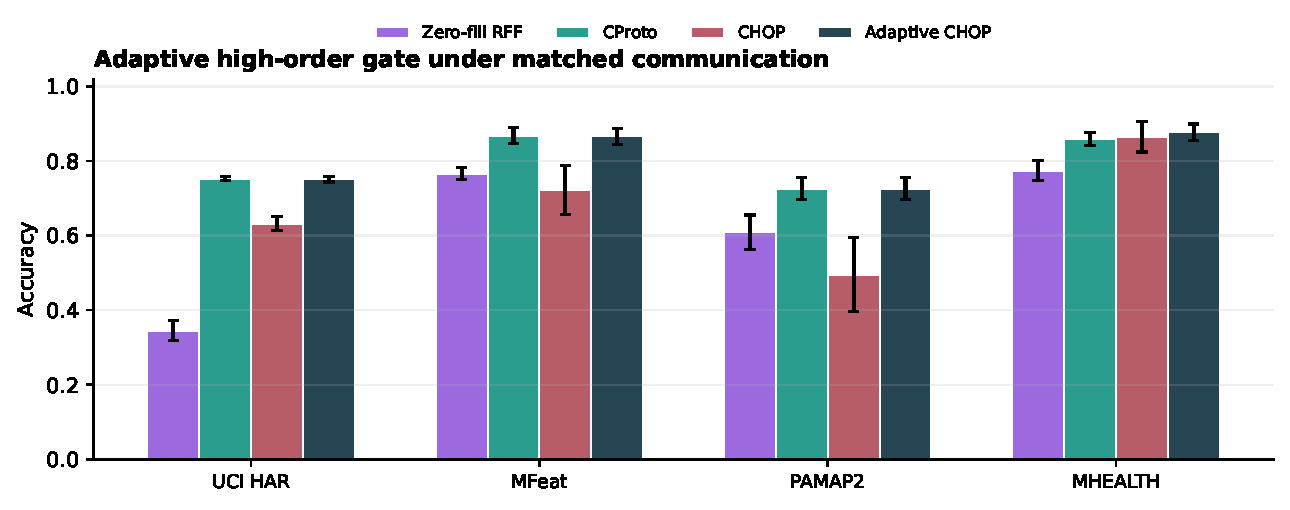
\includegraphics[width=0.95\textwidth]{adaptive_chop_summary.pdf}
    \caption{Adaptive CHOP under matched communication. On low-order-separable or imputation-friendly tasks such as UCI HAR and PAMAP2, the train-only mixture gate falls back to the low-order CProto branch and avoids the pure-CHOP loss. On MHEALTH, where cross-source interactions are stronger, adaptive CHOP is the highest-mean compact equal-byte statistic after ten seeds; the full-dimensional HeMIS baseline is reported separately as a stronger centralized deep-fusion reference.}
    \label{fig:adaptive-chop}
\end{figure*}

\begin{table*}[t]
\centering
\caption{Adaptive CHOP ablation under matched communication. All method columns use the same per-client payload within each dataset. The table separates low-order coverage fusion, random high-order sketches, protocol-selected CHOP, and the train-calibrated mixture/fallback gate.}
\label{tab:adaptive-chop-ablation}
\resizebox{\textwidth}{!}{%
\begin{tabular}{lccccc}
\toprule
Dataset & Zero-fill RFF & CProto & Random HOP & CHOP & Adaptive CHOP \\
\midrule
UCI HAR & 0.344 & 0.753 & 0.616 & 0.632 & 0.752 \\
MFeat & 0.766 & 0.868 & 0.883 & 0.722 & 0.866 \\
PAMAP2 & 0.609 & 0.725 & 0.702 & 0.495 & 0.725 \\
MHEALTH & 0.774 & 0.860 & 0.798 & 0.865 & 0.878 \\
\bottomrule
\end{tabular}%
}
\end{table*}

\begin{table}[t]
\centering
\caption{Adaptive CHOP calibration choices. The gate uses training-only calibration and chooses either the equal-byte CProto fallback or a CHOP-key candidate \(\alpha d_{\mathrm{low}}+(1-\alpha)d_{\mathrm{hop}}\). The \(\alpha=1\) column is a CHOP-key low-order branch rather than a high-order branch.}
\label{tab:adaptive-chop-gate}
\begin{tabular}{lrrrrrrr}
\toprule
Dataset & \(n\) & CProto & \(\alpha=0\) & .25 & .50 & .75 & 1.0 \\
\midrule
UCI HAR & 5 & 4 & 0 & 0 & 0 & 0 & 1 \\
MFeat & 10 & 9 & 0 & 0 & 0 & 0 & 1 \\
PAMAP2 & 5 & 5 & 0 & 0 & 0 & 0 & 0 \\
MHEALTH & 10 & 4 & 0 & 2 & 0 & 0 & 4 \\
\bottomrule
\end{tabular}
\end{table}


Table~\ref{tab:adaptive-chop-ablation} and Fig.~\ref{fig:adaptive-chop} summarize the matched-communication adaptive CHOP behavior, while Table~\ref{tab:adaptive-chop-gate} reports the corresponding training-only gate choices.

PAMAP2 \cite{reiss2012pamap2}, UCI Hydraulic Systems condition monitoring \cite{helwig2015hydraulic}, and WDBC \cite{street1993wdbc} are reported as supplementary checks. PAMAP2 is a larger wearable boundary case: equal-byte CProto/adaptive CHOP reach 0.725, while cross-source CHOP drops to 0.496 and HeMIS reaches 0.753. Hydraulic Systems is useful because it is an industrial condition-monitoring task. On cooler-state classification, compact equal-byte CProto/CHOP reach 0.973/0.977, compared with 0.833 for shared-view RFF and 0.968 for zero-fill RFF; HeMIS/MLP reach 0.997/0.993. The task therefore supports the source-coordinate framing but also shows the expected advantage of full-dimensional trainable models. WDBC is nearly saturated, with learned ridge marginally highest at 0.924. These datasets are boundary checks rather than headline HOP claims.

The strict equal-byte rows in Tables~\ref{tab:if-nonquantum-fusion} and~\ref{tab:if-mfeat-fusion}, together with the MHEALTH, PAMAP2, and Hydraulic Systems appendix tables, address a narrow fairness question: do the compact statistics win simply because they communicate more? Across UCI HAR, MFeat, MHEALTH, PAMAP2, and Hydraulic Systems, CProto, group-balanced CProto, CHOP, or adaptive CHOP is far above equal-byte shared-view RFF controls and is usually competitive with equal-byte zero-fill RFF. Autoencoder, mask-aware MLP, HeMIS, learned-imputation, and late-fusion rows are deliberately not equal-byte rows. They ask a different question: how far can richer full-dimensional reconstruction, trainable missing-modality fusion, or decision fusion go when those tools are allowed? Compact equal-byte-only tables are included in the supplement.

\subsection{Full-Class Heterogeneous Readout}

\begin{table*}[t]
\centering
\caption{Final full-class results under heterogeneous readout. Values are mean accuracy over five seeds; bytes are per client per round.}
\label{tab:masked-fullclass}
\begin{tabular}{lcccc}
\toprule
Dataset & Method & Acc. & 95\% CI & Bytes \\
\midrule
MNIST-10 & \method{}-Masked-HOP & \textbf{0.744} & 0.027 & 24364 \\
MNIST-10 & \method{}-Masked & 0.743 & 0.027 & 20524 \\
MNIST-10 & CHOP, \(K=96\) & 0.739 & 0.030 & 11564 \\
MNIST-10 & CProto, \(K=96\) & 0.738 & 0.030 & 7724 \\
MNIST-10 & shared-observable & 0.695 & 0.018 & 7724 \\
MNIST-10 & FedAdam schema & 0.456 & 0.033 & 7720 \\
MNIST-10 & FedProto schema & 0.412 & 0.029 & 7724 \\
MNIST-10 & SCAFFOLD schema & 0.277 & 0.044 & 15440 \\
MNIST-10 & no-schema & 0.219 & 0.010 & 7724 \\
\midrule
Fashion-10 & \method{}-Masked-HOP & \textbf{0.662} & 0.026 & 24364 \\
Fashion-10 & \method{}-Masked & 0.661 & 0.026 & 20524 \\
Fashion-10 & CHOP, \(K=96\) & 0.660 & 0.027 & 11564 \\
Fashion-10 & CProto, \(K=96\) & 0.660 & 0.027 & 7724 \\
Fashion-10 & shared-observable & 0.656 & 0.019 & 7724 \\
Fashion-10 & FedAdam schema & 0.544 & 0.033 & 7720 \\
Fashion-10 & FedProto schema & 0.522 & 0.037 & 7724 \\
Fashion-10 & SCAFFOLD schema & 0.377 & 0.069 & 15440 \\
Fashion-10 & no-schema & 0.240 & 0.025 & 7724 \\
\midrule
CIFAR-10 & \method{}-Masked-HOP & \textbf{0.454} & 0.004 & 24364 \\
CIFAR-10 & \method{}-Masked & 0.454 & 0.003 & 20524 \\
CIFAR-10 & CHOP, \(K=96\) & 0.451 & 0.004 & 11564 \\
CIFAR-10 & CProto, \(K=96\) & 0.450 & 0.005 & 7724 \\
CIFAR-10 & shared-observable & 0.425 & 0.017 & 7724 \\
CIFAR-10 & FedAdam schema & 0.281 & 0.017 & 7720 \\
CIFAR-10 & FedProto schema & 0.268 & 0.019 & 7724 \\
CIFAR-10 & SCAFFOLD schema & 0.204 & 0.038 & 15440 \\
CIFAR-10 & no-schema & 0.166 & 0.006 & 7724 \\
\bottomrule
\end{tabular}
\end{table*}


Table~\ref{tab:masked-fullclass} reports the final 5-seed full-class image experiments. Correct-schema coverage-aware variants are strongest on MNIST-10, Fashion-10, and CIFAR-10. The largest gap is against schema-incorrect controls, and the advantage remains over schema-aware FedAdam, FedProto, SCAFFOLD, and FedDyn head baselines. The shared-observable row is worth keeping in view: when the common intersection already contains discriminative coordinates, it can be strong, especially on Fashion-10. The result supports the semantic coverage-aware reading of the method, not a universal HOP-gain reading.

\subsection{Missing-View Fusion Controls}

\begin{table*}[t]
\centering
\caption{IF-style heterogeneous fusion controls on full-class datasets. Zero-fill and mask-only are generic missing-observation controls; shared-observable aggregation uses only the intersection observed by every client. Bytes are per client per round.}
\label{tab:if-fusion-controls}
\begin{tabular}{llccc}
\toprule
Dataset & Method & Acc. & 95\% CI & Bytes \\
\midrule
MNIST-10 & Mask-only metadata & 0.099 & 0.003 & 7724 \\
MNIST-10 & Schema zero-fill & 0.692 & 0.020 & 7724 \\
MNIST-10 & No schema & 0.219 & 0.010 & 7724 \\
MNIST-10 & Forced canonical & 0.218 & 0.012 & 7724 \\
MNIST-10 & Shared observables & 0.695 & 0.018 & 7724 \\
MNIST-10 & RFF prototype & 0.407 & 0.032 & 7724 \\
MNIST-10 & CProto & 0.738 & 0.030 & 7724 \\
MNIST-10 & CHOP & 0.739 & 0.030 & 11564 \\
MNIST-10 & QProto-Masked & 0.743 & 0.027 & 20524 \\
MNIST-10 & QProto-Masked-HOP & 0.744 & 0.027 & 24364 \\
\midrule
Fashion-10 & Mask-only metadata & 0.100 & 0.002 & 7724 \\
Fashion-10 & Schema zero-fill & 0.647 & 0.022 & 7724 \\
Fashion-10 & No schema & 0.240 & 0.025 & 7724 \\
Fashion-10 & Forced canonical & 0.242 & 0.026 & 7724 \\
Fashion-10 & Shared observables & 0.656 & 0.019 & 7724 \\
Fashion-10 & RFF prototype & 0.523 & 0.045 & 7724 \\
Fashion-10 & CProto & 0.660 & 0.027 & 7724 \\
Fashion-10 & CHOP & 0.660 & 0.027 & 11564 \\
Fashion-10 & QProto-Masked & 0.661 & 0.026 & 20524 \\
Fashion-10 & QProto-Masked-HOP & 0.662 & 0.026 & 24364 \\
\midrule
CIFAR-10 & Mask-only metadata & 0.100 & 0.001 & 7724 \\
CIFAR-10 & Schema zero-fill & 0.421 & 0.002 & 7724 \\
CIFAR-10 & No schema & 0.166 & 0.006 & 7724 \\
CIFAR-10 & Forced canonical & 0.167 & 0.007 & 7724 \\
CIFAR-10 & Shared observables & 0.425 & 0.017 & 7724 \\
CIFAR-10 & RFF prototype & 0.266 & 0.024 & 7724 \\
CIFAR-10 & CProto & 0.450 & 0.005 & 7724 \\
CIFAR-10 & CHOP & 0.451 & 0.004 & 11564 \\
CIFAR-10 & QProto-Masked & 0.454 & 0.003 & 20524 \\
CIFAR-10 & QProto-Masked-HOP & 0.454 & 0.004 & 24364 \\
\bottomrule
\end{tabular}
\end{table*}


The controls in Table~\ref{tab:if-fusion-controls} separate three possible explanations. \emph{Schema zero-fill} keeps the correct identities but replaces missing measurements with zeros and drops the mask. \emph{Mask-only metadata} keeps only the observed-coordinate pattern. \emph{Shared-observable} aggregation discards every coordinate not seen by all clients. Mask-only stays near chance, so schema metadata alone is not the signal. Zero-fill and shared-observable aggregation can be competitive, but CProto, CHOP, and the full coverage-aware variants remain above them except in the high-overlap Fashion-10 boundary case, where the shared intersection is already informative.

\subsection{High-Order Fusion}

\begin{table}[t]
\centering
\caption{Non-image scientific-fusion stress test with covariance-dominated quantum readout. Classes differ mainly through high-order readout structure, and clients observe heterogeneous observable subsets.}
\label{tab:if-scientific-fusion}
\begin{tabular}{lccc}
\toprule
Method & Acc. & 95\% CI & Bytes \\
\midrule
Mask-only metadata & 0.201 & 0.002 & 1944 \\
Schema zero-fill & 0.627 & 0.030 & 1944 \\
No schema & 0.293 & 0.016 & 1944 \\
Forced canonical & 0.290 & 0.009 & 1944 \\
Shared observables & 0.627 & 0.070 & 1944 \\
FedProto schema & 0.290 & 0.011 & 1944 \\
FedAdam schema & 0.333 & 0.013 & 1940 \\
QProto-Masked & 0.372 & 0.013 & 3864 \\
CProto & 0.358 & 0.028 & 1944 \\
QProto-Masked-HOP & 0.691 & 0.041 & 5784 \\
CHOP & 0.732 & 0.024 & 3864 \\
\bottomrule
\end{tabular}
\end{table}


Table~\ref{tab:if-scientific-fusion} isolates the opposite regime, where high-order statistics should matter. The controlled non-image covariance-sensing task has weak class means, with discriminative information concentrated in high-order readout interactions. Generic missing-view controls are still nontrivial--zero-fill and shared-observable aggregation are around 0.63 accuracy--but CHOP reaches 0.732 at 3864 bytes/client/round, compared with 0.358 for the matched low-order CProto. This is the main HOP/CHOP evidence in the IF narrative. The supplement reports separate PennyLane circuit-generated and synthetic covariance diagnostics; we do not pool those numbers with the main covariance-sensing table.

\subsection{Circuit-Generated Readout Evidence}

Figure~\ref{fig:main-results-overview}D gives the Qiskit Aer circuit-generated readout check across finite-shot, readout-error, depolarizing-noise, and circuit-depth settings; the supplement gives the detailed values. Aer measurement counts are converted into readout features, and the downstream QProto runner disables additional synthetic noise to avoid double counting. This is circuit-level compatibility evidence only, not hardware validation or a claim about physical-device performance.

\subsection{Statistical Tests}

\begin{table*}[t]
\centering
\caption{Paired significance tests for the main experimental claims. Reported values are mean paired accuracy deltas over matched seeds. One-sided paired \(t\)-tests use Holm correction across all tested comparisons; the supplementary table also reports two-sided Holm values.}
\label{tab:if-significance}
\scriptsize
\setlength{\tabcolsep}{3pt}
\renewcommand{\arraystretch}{0.9}
\resizebox{\textwidth}{!}{%
\begin{tabular}{llrrrr}
\toprule
Setting & Comparison & \(n\) & \(\Delta\) acc. & \(d_z\) & Holm \(p_{1s}\) \\
\midrule
MNIST-10 & Masked-HOP - zero-fill & 5 & 0.052 & 4.67 & 0.0059 \\
MNIST-10 & Masked-HOP - shared-observable & 5 & 0.050 & 4.78 & 0.0057 \\
Fashion-10 & Masked-HOP - zero-fill & 5 & 0.015 & 1.86 & 0.0851 \\
Fashion-10 & Masked-HOP - shared-observable & 5 & 0.006 & 0.65 & 0.4422 \\
CIFAR-10 & Masked-HOP - zero-fill & 5 & 0.033 & 8.16 & 0.0009 \\
CIFAR-10 & Masked-HOP - shared-observable & 5 & 0.029 & 1.83 & 0.0851 \\
Covariance sensing & CHOP - zero-fill & 5 & 0.105 & 3.54 & 0.0144 \\
Covariance sensing & CHOP - shared-observable & 5 & 0.106 & 1.53 & 0.1058 \\
Covariance sensing & CHOP - CProto & 5 & 0.374 & 10.35 & 0.0004 \\
MNIST-10 & Masked-HOP - schema-FedProto & 5 & 0.332 & 11.56 & 0.0003 \\
MNIST-10 & Masked-HOP - schema-FedAdam & 5 & 0.288 & 9.27 & 0.0006 \\
Fashion-10 & Masked-HOP - schema-FedProto & 5 & 0.140 & 6.17 & 0.0025 \\
Fashion-10 & Masked-HOP - schema-FedAdam & 5 & 0.118 & 5.04 & 0.0049 \\
CIFAR-10 & Masked-HOP - schema-FedProto & 5 & 0.186 & 10.49 & 0.0004 \\
CIFAR-10 & Masked-HOP - schema-FedAdam & 5 & 0.172 & 10.76 & 0.0003 \\
PennyLane high-order & CHOP - CProto & 3 & 0.199 & 10.72 & 0.0255 \\
PennyLane high-order & CHOP - schema-FedProto & 3 & 0.317 & 25.23 & 0.0063 \\
Qiskit Aer & Masked-HOP - schema-FedProto & 3 & 0.169 & 2.91 & 0.1058 \\
Qiskit Aer & Masked-HOP - FedDyn & 3 & 0.178 & 3.48 & 0.1058 \\
UCI HAR & CProto eq. - zero-fill RFF eq. & 5 & 0.409 & 13.34 & 0.0002 \\
UCI HAR & CProto eq. - shared-view RFF eq. & 5 & 0.362 & 24.84 & \(<0.0001\) \\
MFeat & Group-CProto eq. - zero-fill RFF eq. & 10 & 0.110 & 1.89 & 0.0031 \\
MFeat & Group-CProto eq. - shared-view RFF eq. & 10 & 0.182 & 4.17 & \(<0.0001\) \\
MHEALTH & CHOP eq. - CProto eq. & 10 & 0.005 & 0.09 & 1.0000 \\
MHEALTH & CHOP eq. - zero-fill RFF eq. & 10 & 0.091 & 1.05 & 0.0579 \\
MHEALTH & CHOP eq. - mask-aware MLP & 10 & 0.005 & 0.07 & 1.0000 \\
UCI HAR & Adaptive CHOP - CHOP eq. & 5 & 0.120 & 4.82 & 0.0057 \\
MFeat & Adaptive CHOP - CHOP eq. & 10 & 0.144 & 1.62 & 0.0071 \\
PAMAP2 & Adaptive CHOP - CHOP eq. & 5 & 0.230 & 2.74 & 0.0269 \\
\bottomrule
\end{tabular}%
}
\end{table*}


Table~\ref{tab:if-significance} reports paired seed-level tests for the main claims. We use one-sided paired tests for the directional hypotheses and apply Holm correction across the reported comparisons. Fashion-10 against shared-observable and the Qiskit Aer rows in the full supplementary table remain underpowered or not significant after correction. The Aer rows use the matched three-seed backend compatibility comparisons, whereas the robustness sweep in Fig.~\ref{fig:main-results-overview}D uses five seeds per noise setting. The statistically strongest parts of the paper are the full-class heterogeneous-fusion comparisons, the real non-quantum missing-view comparisons, and the covariance-dominated high-order fusion comparisons.

\section{Discussion and Limitations}

\subsection{Main Empirical Message for Information Fusion}

The main empirical lesson is that comparability has to be specified before fusion. Quantum readout makes the point concrete, but nothing in the failure mode is uniquely quantum: the same ambiguity appears when clients expose source-specific coordinates, local orders, missing views, or unequal measurement budgets. The no-schema, forced-canonical, wrong-schema, zero-fill, and mask-only controls correspond to familiar fusion failures--uncalibrated sources, incorrect alignment, simple imputation, and metadata-only fusion. Their behavior is the reason we treat the schema as part of the protocol rather than as bookkeeping.

The real-data benchmarks put that claim outside the quantum setting. UCI HAR, UCI Multiple Features, MHEALTH, PAMAP2, Hydraulic Systems, and WDBC cover phone sensors, wearable blocks, industrial condition monitoring, multi-view digit features, and biomedical measurements. In these settings, coverage-aware QProto is competitive with PCA, ridge and autoencoder imputation, mask-aware pooled MLP, and view-wise late fusion, while it is consistently stronger than equal-byte shared-view RFF controls. HeMIS is stronger on several tasks when trained as a full-dimensional missing-modality classifier; we view this as a useful boundary, not a contradiction, because QProto is designed for compact protocol statistics under source-identity and payload constraints. Put differently, QProto is not a substitute for HeMIS or MLP-style missing-modality learners when centralized full-dimensional training is available. It addresses the complementary protocol question that those models usually take for granted: whether distributed source coordinates have shared semantic identities and can be communicated as compact federated statistics. Multiple Features shows why source groups should not be treated as anonymous coordinates when view dimensionalities differ. MHEALTH is the clearest real interaction-heavy case for adaptive CHOP. PAMAP2, Hydraulic Systems, MFeat, and HAR are the counterweight: there, low-order or calibrated mixtures are safer than blind HOP. WDBC is nearly saturated. Together these cases give a narrower but cleaner claim: QProto is a schema/value/count fusion protocol for settings where source identity, coverage, and communication constraints would otherwise make aggregation ambiguous.

\subsection{Role of HOP}

The high-order module should be used selectively. The full-class image experiments and the real UCI HAR/MFeat/PAMAP2/WDBC tasks are largely low-order or coverage-separable after schema alignment; CProto or group-balanced low-order fusion is usually the safer compact statistic. MHEALTH, the PennyLane high-order readout, the covariance-sensing task, and the synthetic covariance benchmark contain stronger second-order or cross-source structure, and mask-aware HOP becomes more useful there. Adaptive CHOP turns this observation into a rule: it improves over pure CHOP on HAR, MFeat, and PAMAP2, and on the ten-seed MHEALTH run it gives the highest mean among compact equal-byte statistics by choosing non-CProto candidates on 6/10 seeds. The key is that HOP is still part of the comparability protocol. Random-key HOP is weak on UCI HAR and WDBC and gives no gain over random-key CProto on MHEALTH; on MFeat, random-key low-order CProto is itself strong, so we do not use that benchmark to claim key-selection superiority. Cross-source CHOP helps only when anchor-selected keys correspond to meaningful source interactions.

\subsection{Role of Shot-Variance Shrinkage}

Shot-variance shrinkage remains a reliability hook rather than a headline method. In highly non-IID label splits, downweighting noisy clients can also suppress rare class evidence. A more useful version would be class-aware or calibration-aware, instead of a single client-level reliability scalar.

\subsection{Hardware and Backend Limitations}

The implementation currently covers backend-agnostic simulated readouts, PennyLane circuit-generated readouts, and Qiskit Aer noisy readouts. These are compatibility checks, not hardware validation. A small IBM hardware demonstration with the same schema adapter and a 2-class or 4-class task would be a natural next step if low-cost access is available. The code already includes a Qiskit circuit/count-to-readout path: it builds one circuit per observable, converts bit counts into expectation values, and writes the same precomputed-readout format used by the main experiments. In this environment the path was verified on Aer fallback only, because IBM Runtime is not installed and no token is available.

\subsection{Dataset Scope}

The dataset coverage is broad but not exhaustive. The experiments include first-four-class diagnostics and full ten-class experiments for MNIST, Fashion-MNIST, and CIFAR-10 features, scale and observable-overlap sweeps, real UCI HAR, UCI Multiple Features, MHEALTH, PAMAP2, Hydraulic Systems, and WDBC missing-view benchmarks, and controlled non-image high-order fusion tasks. Gas Drift appears only in the supplement as a boundary check: even with cross-sensor HOP pair selection, low-order or learned baselines are stronger, so it is not used as HOP evidence. Remote sensing or a larger industrial monitoring benchmark would further reduce the chance that the paper is read as primarily quantum-computing-specific.

\section{Conclusion}

We presented \method, a protocol-defined semantic fusion framework for heterogeneous source-coordinate aggregation. Quantum measurement motivates the formalism, but the broader issue is missing-view source fusion: before clients upload prototypes, the protocol must say what makes their statistics comparable. With a public value-and-mask schema, coverage-aware class statistics, and optional high-order sketches, \method\ lets the server fuse evidence across different source coordinates.

Across image experiments, real missing-view benchmarks, quantum-backend compatibility checks, and controlled high-order tasks, correct schema binding and coverage-aware fusion outperform schema-incorrect, zero-fill, shared-view, FedOpt/FedProto, and equal-byte RFF controls under the tested protocols. Strong learned imputation, autoencoder imputation, mask-aware MLP, HeMIS-style fusion, and late fusion define the full-dimensional boundary; they can match or exceed protocol prototypes when trainable reconstruction or missing-modality classifiers are allowed. Under compact communication, schema-aware prototypes remain much stronger than shared-view compression and usually competitive with equal-byte zero-fill fusion. HOP/CHOP is similarly conditional: it is central when evidence is covariance-dominated or cross-source-interaction-driven, while low-order coverage-aware or group-balanced fusion is preferable when first-order evidence is already strong. The contribution is therefore not a universal missing-modality learner, but a protocol argument: semantic coordinate identity, missingness, coverage, and payload should be first-class objects in QFL and heterogeneous-source FL.

\section*{Data and Code Availability}

All experiments are designed to be reproducible from public datasets or generated readout files. MNIST, Fashion-MNIST, CIFAR-10 feature exports, UCI HAR, UCI Multiple Features, MHEALTH, PAMAP2, Hydraulic Systems, WDBC, and Gas Drift boundary-check commands are listed in the supplementary material. The Qiskit Aer and PennyLane studies are circuit-generated readout compatibility checks; no paid IBM hardware data are used. A review source and code archive with fixed seeds, scripts, configuration files, selected result summaries, payload accounting, and cached-feature checksums is submitted as supplementary material. A public repository will be released upon acceptance.

\section*{CRediT Authorship Contribution Statement}

Leyuan Zhang: Conceptualization, Methodology, Software, Validation, Formal analysis, Investigation, Writing -- original draft, Visualization. Yang Long: Supervision, Conceptualization, Methodology, Writing -- review \& editing, Project administration.

\section*{Funding}

Leyuan Zhang acknowledges financial support from the China Scholarship Council (CSC). The funder had no role in the study design, data collection, analysis, interpretation, manuscript preparation, or decision to submit the article for publication.

\section*{Declaration of Competing Interest}

The authors declare that they have no known competing financial interests or personal relationships that could have appeared to influence the work reported in this paper.

\section*{Declaration of Generative AI and AI-Assisted Technologies in the Writing Process}

During the preparation of this work, the authors used AI-assisted tools to support language polishing, editorial organization, and consistency checks. The authors reviewed and edited the content as needed and take full responsibility for the content of the article.


\FloatBarrier
\bibliographystyle{elsarticle-num}
\bibliography{references}

\end{document}


